\chapter{Bayesian learning for DPPs}


So far we have seen two different estimation techniques for the parameters of DPPs. Although we proved that they provide reasonable estimators in the sense that they are consistent, they have some drawbacks. For example we have seen that the MLEs for the different parameters do not exist in general, let alone that they are impossible to compute in reality. Further
%Firstly, we saw that the maximum likelihood estimator does not exist in general and in some cases one needs a fairly high amount of samples to ensure that it does. Secondly 
all of the estimators presented so far are point estimators, i.e. they return a single value for the desired parameter. Obviously this does not allow to capture any uncertainties that the estimation of the parameter has. % and we have already seen in that the selection of the most possible outcome -- in this case the MLE -- might not yield a very typical one for a given random variable.
Those are some reasons to consider the Bayesian approach of parameter estimation where the goal is to give a distribution -- called the posterior -- of the parameter that should be estimated instead of a single value. This can also help to overcome some -- maybe even all of the problems mentioned above.

At first we will present the general concept of Bayesian parameter estimation and will then turn towards the question of computability of the posterior distribution. %Since the normalisation constant of the 
For this we will follow the approach of \cite{affandi2014learning} and turn towards the popular Markov chain Monte Carlo (MCMC) methods. We quickly explain their philosophy and how they can be used to approximate the posterior distribution of the parameter one wishes to estimate.

\section{Bayesian approach to parameter estimation}

For the introduction of the general Bayesian setup we pursue like in \cite{rice2006mathematical}. Just like in the case of MLE we want to estimate %the underlying density of 
a parameter \(\theta\in\Theta\) based on
 some realisations \(x = (x_1, \dots, x_n)\) of random variables \(X = (X_1, \dots, X_n)\). 
 %out of a parametric family
%\[\mathcal F = \Big\{ f_{X| \Theta}(\cdot |\theta) \mid \theta\in\Theta\Big\}\]
%of probability densities with respect to \(\mu^n\coloneqq\prod_{i=1}^n\mu(\mathrm d x_i)\).
 This time, however, we are not interested in returning a single value \(\theta\) because this would be a vast simplification of the stochastic nature of the estimator. Thus, we want to obtain a probability distribution over whole parameter space \(\Theta\) that indicates how likely the parameters are to have caused the observed data. In order to present the procedure we will introduce the frame we will work in.

\begin{emp}[Setting]
Let \(\Theta\) be a measurable space and \(\nu\) be a measure on \(\Theta\). Let \(f_\Theta\colon \Theta\to[0, \infty]\) be a probability density with respect to \(\nu\), i.e.
\[\int\limits_{\Theta} f_\Theta(\theta)\nu(\mathrm{d}\theta) = 1\]
which we will call the \emph{prior} distribution of the parameter \(\theta\).\footnote{The requirement of \(f\) being a probability density can easily be loosened. In fact if it has finite integral it is obvious that the normalisation cancels in the definition \eqref{post} of the posterior and even if it has infinite integral, \eqref{post} might still give a probability density.} Further let
\[\mathcal F = \Big\{ f_{X| \Theta}(\cdot |\theta) \;\big\lvert\; \theta\in\Theta\Big\}\]
by a family of probability densities with respect to \(\mu^n\coloneqq\prod_{i=1}^n\mu(\mathrm d x_i)\).
\end{emp}

Usually the prior distribution will encode some perceptions or prior knowledge we might have of the parameter. For example if we are trying to estimate a physical constant that we know has to be positive, then it is reasonable to select a prior that has its whole mass on the positive real line. However, there is no clear set of rules how one can select a suitable prior to a given problem. %Further we will see how the prior gives a way of regularisation in the sense that 

%To obtain the distribution of \(\theta\) given the observations \(x\) we will first construct the joint density of both parameters and then take the marginal distribution of \(\theta\).
The density \(f_{X|\Theta}(x|\theta)\) describes how likely the observations are under the parameter \(\theta\) and we want to find an expression of how likely the parameter \(\theta\) is under the observations \(x\). %and \(f(\theta)\) 
In order to obtain this, we will work with the joint density
\[f_{X, \Theta}(x, \theta) = f_{X|\Theta}(x|\theta) f_\Theta(\theta) \quad \text{with respect to } \mu^n \times \nu \]
and condition this onto \(x\). This yields
\begin{equation}\label{post}
\begin{split}
f_{\Theta| X}(\theta|x) = \frac{f_{X, \Theta}(x, \theta)}{\int_{\Theta} f_{X, \Theta}(x, \theta)\nu(\mathrm{d}\theta)} = \frac{f_{X|\Theta}(x| \theta) f_\Theta(\theta)}{\int_{\Theta} f_{X, \Theta}(x, \theta)\nu(\mathrm{d}\theta)}.
\end{split}
\end{equation}

\begin{defi}[Posterior distribution]
The density \(f_{\Theta|X}\) is called the \emph{posterior distribution} of the parameter \(\theta\) given the data \(x\). Further we call the normalisation constant
\[f(x|\mathcal F) \coloneqq \int_{\Theta} f_{X, \Theta}(x, \theta)\nu(\mathrm{d}\theta) \]
the total probability of the data \(x\) under the model \(\mathcal F\).
\end{defi}

%From now on we will assume -- just like in the case of MLE -- that our observations are independent and identically distributed and hence their joint distribution factorises and we obtain
%\[f_{\Theta| X}(\theta|x) \propto f_\Theta(\theta) \prod_{i=1}^n f_{X|\Theta}(x_i| \theta)\]
%recent\todo{add remark on intuition?}
%This posterior density is already the object which is supposed to give us the information of the distribution of the parameter given the data \(x\). It is proportional to the likelihood \(f_{X|\Theta}(x|\theta)\) of the occuring data times the prior \(f_\Theta(\theta)\) which can be understood in the way, that 

First we will convince ourselves that the approach of calculating a posterior distribution is a generalisation of the MLE in a lot of cases.

\begin{emp}[Comparison to MLE]
Maybe one feels slightly uncomfortable with the need to choose a prior distribution and it turns out that this is in fact a difficult step that has to be taken with a certain amount of care. However, we could pretend for one moment to be completely ignorant in the sense that we do not know anything about the parameter and hence we don�t feel in the position to propose a reasonable prior. Then we could simply choose the uniform distribution as a prior -- given it exists\footnote{Even it doesn�t one can still define the prior density to be constant and hope that the posterior is a probability density.} -- and would obtain
\[f_{\Theta| X}(\theta|x) \propto f_{X|\Theta}(x|\theta). \]
Hence we can regain the MLE from our posterior distribution since it is just the mode, i.e. the maximiser of the posterior density. This relation to the MLE can be seen in Figure \ref{fig:4.1}. Hence, the Bayesian approach is a more general tool than MLE and allows to capture the randomness of the parameter \(\theta\). This is desirable since  we have seen that the mode is not always a vey typical outcome of a random variable. %\todo{cite}.
\begin{figure}[h!]
	\centering
	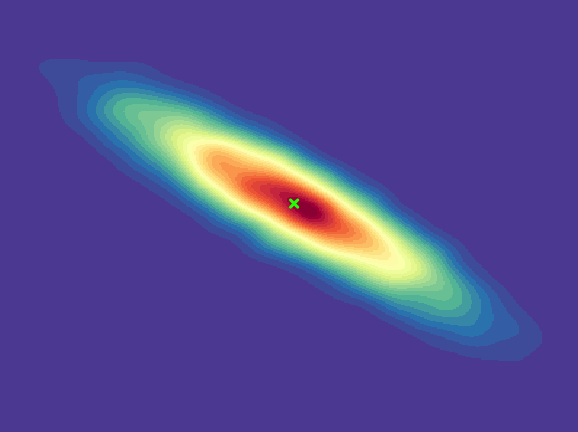
\includegraphics[width=0.6\textwidth]{figures/heatmap-log-linearity-SliceSampling-new-3}
%	\tag{1}
	\caption{Approximated posterior density of the two dimensional log linearity constant of a two dimensional DPP with a uniform distribution as a prior. The MLE estimator is marked green and is at the mode of the distribution.}
	\label{fig:4.1}
\end{figure}

A further advantage over the MLE is that it might be possible to computationally approximate the posterior density, but not the MLE. This is typically the case if the log likelihood function is not concave, like in the setting of the MLE of the whole elementary kernel \(L\). In fact the only hard step in the calculation of the posterior \eqref{post} is the computation of the normalisation constant
\[\int\limits_{\Theta} f_{X,\Theta}(x, \theta) \nu(\mathrm{d}\theta). \]
This can often not be performed efficiently but the Markov chain Monte Carlo methods introduced later will yield an approximation of the posterior without the need to compute the normalisation constant.
\end{emp}

\begin{emp}[Regularisation through the prior]
The prior density is very closely related to the regulariser introduced in the section about maximum likelihood estimation. In fact the mode of the posterior \(f_{\Theta|X}\) is nothing else but the maximiser of 
\[\log(f_{\Theta|X}) = \mathcal L + F\]
where \(F = \log(f_\theta)\) and hence nothing else but a regularised MLE. In fact if \(F\) is a regularisation and \(\exp(F)\) is integrable with respect to \(\mu\), then one can choose \(f_\Theta\propto \exp(F)\) as a prior density. Hence the proposition of a prior and a regulariser are equivalent in a wide variety of cases, but again, the posterior density encodes much more information than just the location of its mode which is the regularised MLE.

%\todo{regularisation of noise}

%We will assume that we are in the setting of the estimation of the log linearity constant \(\theta\in\mathbb R^M\) and we will define the prior density to be the standard normal density on \(\mathbb R^M\). Further let \(Y_1, \dots, Y_n\) be some data such that the MLE \(\hat\theta_n\) does not consist. Recall that if this is the case, one of the items \(i\in\mathcal Y\) is either present in none or in all of the observations and hence the quality estimation would (formally) be \(0\) or \(\infty\). Therefore, the respective log linearity constant might not exist in \(\mathbb R^M\).

%Of course we have seen in the section about coercivity of the log likelihood functions that the probability for this to happen tends to zero with increasing sample size, however in practice it might not be possible to obtain more samples. In this scenario the maximum likelihood approach fails but the posterior density \eqref{post2} still exists. One way of explaining this is that the prior assigns small values to parameters far away from zero. Hence, the prior can be seen as a kind of regularisation since it penalises parameters that lead to very irregular models. In our case irregular means that the log linearity constant is big which implies that one quality is either very high or close to zero. Having a high quality corresponds to the model almost not being a \(L\)-ensemble any more and having quality zero means that the model can not be expressed any more through log linear qualities.

%In similar fashion a suitable prior distribution might be used to make the parameter estimation more stable in the case that the data is perturbed by some noise. However, this would need some further investigation. %\todo{work on this.}
\end{emp}

%\begin{enumerate}
%\item explain general procedure and say something about intuition
%\item explain the benefits, namely:
%\begin{enumerate}
% \item can capture uncertainty
% \item might me more feasible
% \item is an extension, at least if there is a uniform distribution on the parameter space
%\item offers a method for regularisation, i.e. will sometimes work if MLE doesn�t (properly) work due to statistical fluctuations like overfitting of noise
%\end{enumerate}
%\item 
%\end{enumerate}

\begin{emp}[Bayesian approach without prior]
We have seen that the prior is nothing else but a regularisation of the likelihood and since MLE can be carried out without regularisation it is natural to ask whether the Bayesian approach works without a prior. We have seen that if there is a uniform distribution on the parameter space, the unregularised MLE corresponds to the uniform distribution as a prior. So the question is what changes if we propose \(f_\Theta = 1\) as a prior if there is no uniform distribution, or more generally what happens if the prior \(f_\Theta\) has infinite integral.

In this case, the unnormalised posterior distribution 
\begin{equation}\label{genpost}
\mathfrak{f}(\theta) = f_{X|\Theta}(x| \theta) f_\Theta(\theta)
\end{equation}
might not have finite integral and can therefore not be normalised. Hence the posterior can not be seen as a probability density, but the generalised form \eqref{genpost} still exists. If we use the constant prior \(f_\Theta=1\), the generalised posterior \(\mathfrak{f}(\theta)\) is just the observation probability (or density if \(\mathcal X\) is continuous) of the data \(x\) under the parameter \(\theta\).
%We will use this approach later to remove the effect of a prior that influences the posterior and also the MLE.
\end{emp}

\subsubsection*{Expression of the posterior for DPPs}

Now we will express the posterior in the case of DPPs under the following conditions.

\begin{emp}[Setting]
Let \((\Theta, \nu)\) be a measure space and \(L(\theta)\in\mathbb R^{N\times N}_{\text{sym}, +}\) be an elementary kernel for every \(\theta\in\Theta\). Further we assume that we have independent realisations \(A_1, \dots, A_n\) of a  \(L\)-ensemble.
\end{emp}

Typically the parametrisations \(\theta\mapsto L(\theta)\) will be one of the three parametric models in III.2.1, i.e. \(\theta\) will either be the whole kernel itself, the quality vector or the log linearity constant of the qualities and \(L(\theta)\) the associated elementary kernel.

The independence relation leads to a factorisation of the density and we obtain the following expression for the posterior density
\begin{equation}\label{post2}
f(\theta|A_1, \dots, A_n) \propto f_\Theta(\theta) \prod_{i=1}^n f(A_i|\theta) = f_\Theta(\theta) \prod_{i=1}^n \frac{\det(L(\theta)_{A_i})}{\det(L(\theta) + I)}
\end{equation}
where we dropped some indices of the density functions. % in slight abuse of notation.

Unfortunately the normalisation constant
\begin{equation}\label{norma}
\int\limits_{\Theta} f(\theta|A_1, \dots, A_n)\nu(\mathrm{d}\theta) = \int\limits_{\Theta} f_\Theta(\theta) \prod_{i=1}^n \frac{\det(L(\theta)_{A_i})}{\det(L(\theta) + I)}\nu(\mathrm{d}\theta)
\end{equation}
can neither be computed analytically nor numerically in an efficient way since the evaluation of this density involves the computation of the determinant of \(N\times N\) matrices. This problem can be solved through the powerful method of Markov chain Monte Carlo simulation that allow to approximate a distribution with only the knowledge of its unnormalised density. But before we introduce those methods, we quickly explain how the Bayesian approach offers a possibility of regularisation and hence can be used to increase the noise sensitivity of the parameter estimation.

\subsubsection{Model selection using the Bayes factor}

In this paragraph we will quickly touch on how the Bayesian approach can be used to compare two different models, i.e. two different parametric families \(\mathcal F_1\) and \(\mathcal F_2\) including two different priors \(f_{\Theta_1}\) and \(f_{\Theta_2}\). For this we will work in the following setup.

\begin{emp}[Setting]
Let \(\Theta_1, \Theta_2\) be measurable spaces and \(\nu_i\)  measures on \(\Theta_i\) for \(i=1, 2\). Let \(f_{\Theta_i}\colon \Theta_i\to[0, \infty]\) be probability densities with respect to \(\nu_i\), i.e.
\[\int\limits_{\Theta_i} f_{\Theta_i}(\theta)\nu_i(\mathrm{d}\theta) = 1 \quad \text{for } i = 1, 2.\]
Further let
\[\mathcal F_i = \Big\{ f_{X| \Theta_i}(\cdot |\theta) \;\big\lvert\; \theta\in\Theta_i\Big\}\]
by a family of probability densities with respect to \(\mu^n\coloneqq\prod_{i=1}^n\mu(\mathrm d x_i)\).
\end{emp}

The goal is now two compare which model \(\mathcal F_i\) in combination with the corresponding prior describes the phenomenon better given some data \(x\). For this we follow \cite{kass1995bayes} and introduce the \emph{Bayes factor} of the two models given the data \(x\) through
\[K \coloneqq K(\mathcal F_1, \mathcal F_2| x) \coloneqq\frac{f(x|\mathcal F_1)}{f(x|\mathcal F_2)} = \frac{\int_{\Theta_1} f_{X| \Theta_1}(x| \theta) f_{\Theta_1}(\theta)\nu_1(\mathrm{d}\theta)}{\int_{\Theta_2} f_{X| \Theta_2}(x| \theta) f_{\Theta_2}(\theta)\nu_2(\mathrm{d}\theta)}. \]
This is nothing but the ratio of the total probabilities of the data \(x\) under the respective models. If this ratio is big, the model \(\mathcal F_1\) including its prior can be seen as a better description of the data compared to the second model. There is no clear definition on when the ratio can be seen as big enough to say this, but the following guidelines in Table \ref{tab:BayesFactor} were proposed in \cite{kass1995bayes}.

\begin{table}
\centering
\begin{tabular}{ |c|c| } 
 \hline
  Value for \(K\) & Interpretation \\ \hline
 \(1 - 3.2\) & Only worth a bare mention \\ \hline
 \(3.2 - 10\) & Substantial \\ \hline
 \(10 - 100\) & Strong \\ \hline
 \(>100\) & Decisive \\ \hline
\end{tabular}
\caption{Interpretation of how strongly different values of \(K\) imply that the first model is a better description of the data than the second one.} \label{tab:BayesFactor}
\end{table}


%\begin{emp}[Regularisation through the prior]
%The prior density is very closely related to the regulariser introduced in the section about maximum likelihood estimation. In fact 

%We will assume that we are in the setting of the estimation of the log linearity constant \(\theta\in\mathbb R^M\) and we will define the prior density to be the standard normal density on \(\mathbb R^M\). Further let \(Y_1, \dots, Y_n\) be some data such that the MLE \(\hat\theta_n\) does not consist. Recall that if this is the case, one of the items \(i\in\mathcal Y\) is either present in none or in all of the observations and hence the quality estimation would (formally) be \(0\) or \(\infty\). Therefore, the respective log linearity constant might not exist in \(\mathbb R^M\).

%Of course we have seen in the section about coercivity of the log likelihood functions that the probability for this to happen tends to zero with increasing sample size, however in practice it might not be possible to obtain more samples. In this scenario the maximum likelihood approach fails but the posterior density \eqref{post2} still exists. One way of explaining this is that the prior assigns small values to parameters far away from zero. Hence, the prior can be seen as a kind of regularisation since it penalises parameters that lead to very irregular models. In our case irregular means that the log linearity constant is big which implies that one quality is either very high or close to zero. Having a high quality corresponds to the model almost not being a \(L\)-ensemble any more and having quality zero means that the model can not be expressed any more through log linear qualities.

%In similar fashion a suitable prior distribution might be used to make the parameter estimation more stable in the case that the data is perturbed by some noise. However, this would need some further investigation. %\todo{work on this.}
%\end{emp}

\section{Markov chain Monte Carlo methods}

The method of Markov chain Monte Carlo (MCMC) simulation arose almost as early as the Monte Carlo\footnote{A legend has it that the name Monte Carlo was given to the work of von Neumann and Ulam %in Los Alamos 
by a colleague referring to Ulam�s uncle who lost a significant amount of money gambling in the Monte Carlo casino in Monaco.} simulations itself and since then a rich theory has been established and a broad range of applications have been found. However, we can only give a short overview over the basic principles and refer to \cite{meyn2012markov} for an introduction of Markov chain theory and to \cite{robert2013monte} for a survey on (Markov chain) Monte Carlo methods. 

We motivated MCMC methods for the approximation of a distribution \(\pi\) under the knowledge of its unnormalised density. In the nutshell the idea is to construct an ergodic Markov chain \((X_n)_{n\in\mathbb N}\) with stationary distribution \(\pi\), i.e. such that one has
\[ \hat{\mathbb P}_n =\frac1n \sum_{i=1}^n \delta_{X_n} \xlongrightarrow{n\to\infty} \pi \]
almost surely in the weak sense. 
This Markov chain can then be simulated using Monte Carlo methods and the associated empirical measure \(\hat{\mathbb P}_n\) will be approximations of \(\pi\). However, to explain this in more detail we need to recapture some notions of Markov chains.

% The reason nables amongst other things to sample from or to approximate a distribution without knowing the normalisation constant.

\subsection{Reminder on Markov chains}

We will provide an extremely short presentation of only those results that we will use to explain the core of MCMC methods. However, this will not contain any proofs and hence it can not replace the study of the already mentioned text books. %Further it will be of great benefit for the reader to be familiar with the basic notions and  of stochastic processes and Markov chains.

Let in the following \((\mathcal X, \mathcal B(\mathcal X))\) be a measurable space.


\begin{defi}[Markov chain]
\begin{enumerate}
\item A \emph{transition kernel} is a function \[K\colon\mathcal X\times\mathcal B(\mathcal X)\to[0, 1]\] such that
\begin{enumerate}
\item \(K(x, \cdot)\) is a probability measure for every \(x\in\mathcal X\) and
\item \(K(\cdot, A)\) is measurable for every \(A\in\mathcal B(\mathcal X)\).
\end{enumerate}
\item A \emph{Markov chain} with values in \(\mathcal X\) and transition kernel \(K(\cdot, \cdot)\) is a collection \((X_n)_{n\in\mathbb N}\) of \(\mathcal X\) valued random variables such that
\begin{equation}\label{MC}
\mathbb P\big(X_0\in A_0, \dots, X_n\in A_n\big) = \int\limits_{A_0} \gamma(\mathrm{d}x_0) \int\limits_{A_1} K(x_0, \mathrm{d}x_1) \cdots \int\limits_{A_n} K(x_{n-1}, \mathrm{d}x_n)
\end{equation}
for all \(A_1, \dots, A_n\in\mathcal B(\mathcal X)\) where \(\gamma\) denotes the distribution of \(X_0\).
\end{enumerate}
\end{defi}

We will call \(\gamma\) the \emph{initial} or \emph{starting distribution} of the Markov chain and will denote the distribution of this Markov chain by \(\mathbb P_\gamma\) and the expectation with respect to it by \(\mathbb E_\gamma[\cdot]\). Further an easy application of Kolmogorov�s consistency theorem implies that there is a measure \(\mathbb P_\gamma\) on the \emph{path space} \(\mathcal X^{\mathbb N}\) that satisfies \eqref{MC} which shows the existence of a Markov chain given a
%one can show that there is a Markov chain for any given %we note that we obtain a Markov chain with
transition kernel \(K\) and initial distribution \(\gamma\) (cf. \cite{le2016brownian}). %by taking \(X_0\) distributed according to \(\gamma\) and \(X_{n+1}\) distributed according to \(K(X_n, \cdot)\) for \(n = 0, 1, \dots\).
 If the initial distribution is deterministic, i.e. \(\gamma = \delta_x\) for one \(x\in\mathcal X\), then we also write \(\mathbb P_x\) for the distribution of the Markov chain.
We close this paragraph by introducing the notation
\[K^n(x, A) \coloneqq \mathbb P_x(X_n\in A) \]
which is consistent with \eqref{MC} for \(n=1\).

%\begin{enumerate}
% \item Definition
%\item irreducibility
% \item existence of stationary distributions
%\item reversibility
%\item detail-balance
%\item Ergodicity 
%\item idea of MCMC
%\end{enumerate}

\subsubsection*{Irreducibility, recurrence and existence of stationary distributions}

From now on we will fix a reference measure \(\mu\) on \(\mathcal X\).

\begin{defi}[Irreducibility and recurrence]
\begin{enumerate}
\item We say a Markov chain is \emph{\(\mu\) irreducible} if for every \(A\in\mathcal B(\mathcal X)\) with \(\mu(A)>0\) there is an index \(n\in\mathbb N\) such that
\[\mathbb P_x(X_n\in A) = K^n(x, A) > 0 \quad \text{for all } x\in\mathcal X. \]
\item A Markov chain \((X_n)_{n \in\mathbb N}\) is called \emph{recurrent} if
\begin{enumerate}
\item there is a measure \(\mu\) on \(\mathcal B(\mathcal X)\) such that \((X_n)\) is \(\mu\)-irreducible and
\item for every \(A\in\mathcal B(\mathcal X)\) with \(\mu(A)>0\) the expected number of visits of \(A\) is infinite, i.e.
\[\mathbb E_x\left[\left\lvert \left\{ n\in\mathbb N \mid X_n\in A\right\} \right\rvert\right] = \infty \quad \text{for every } x\in A.\]
\end{enumerate}
\item A Markov chain is called \emph{Harris recurrent} if it is recurrent and the number of visits is almost surely infinite, i.e. for any \(A\in\mathcal B(\mathcal X)\) with \(\mu(A)>0\) we have
\[\mathbb P_x\left(\left\lvert \left\{ n\in\mathbb N \mid X_n\in A\right\} \right\rvert = \infty\right) = 1 \quad \text{for every } x\in A.\]
\end{enumerate}
\end{defi}

\begin{defi}[Stationary distributions]
Let \(\pi\) be a measure on \(\mathcal B(\mathcal X)\). We call \(\pi\) an \emph{invariant} or \emph{stationary distribution} of a Markov chain with kernel \(K\), if \(X_{n+1}\) is distributed according to \(\pi\) whenever \(X_n\) is distributed according to \(\pi\). This is equivalent to
\[\pi(A) = \int\limits_{\mathcal X} K(x, A)\pi(\mathrm d x) \quad \text{for all } A\in\mathcal B(\mathcal X). \]
\end{defi}

\begin{theo}[Existence of stationary distributions]
If \((X_n)_{n\in\mathbb N}\) is a recurrent Markov chain, there exists an invariant \(\sigma\)-finite measure which is unique up to a multiplicative factor.
\end{theo}

\subsubsection*{Convergence to the stationary distribution and ergodicity}

We will not introduce the notion of periodic and aperiodic Markov chains here, because it would distract us from our actual goal. However, we still present the following result that only holds for aperiodic Markov chains and refer to \cite{meyn2012markov} for further information. The reason why we present the theorem is that it explains how one can approximately sample from the stationary distribution of a Markov chain, namely it says that the distribution of \(X_n\) converges to the invariant distribution.

\begin{theo}[Convergence to stationary distribution]
Let \((X_n)_{n\in\mathbb N}\) be a Harris recurrent and aperiodic Markov chain with stationary distribution \(\pi\). Let further \(\gamma_n\) be the distribution of \(X_n\), then we have
\[\left\lVert \gamma_n - \pi \right\rVert_{TV} \xlongrightarrow{n\to\infty} 0 \]
non increasing. Here \(\left\lVert \cdot \right\rVert_{TV}\) denotes the total variation of a measure
\[\left\lVert \mu \right\rVert_{TV}\coloneqq \sup_{\mathcal E}\sum\limits_{E\in\mathcal E} \left\lvert \mu(E) \right\rvert\]
where the supremum is taken over all finite families of disjoint measurable sets.
\end{theo}

\begin{theo}[Ergodic theorem]\label{ergTheo}
Let \((X_n)_{n\in\mathbb N}\) be a Harris recurrent Markov chain with stationary probability distribution \(\pi\), then \((X_n)_{n\in\mathbb N}\) is \emph{ergodic}. This means that if %\(\gamma_n\) be the distribution of \(X_n\), then we have
\[\hat{\mathbb P}_n \coloneqq \frac1n \sum_{i=1}^n \delta_{X_i} \]
is the empirical measure, we have almost surely have
\begin{equation}\label{ergo}
\int\limits_{\mathcal X} f(x) \hat{\mathbb P}_n(\mathrm dx) \xlongrightarrow{n\to\infty} \int\limits_{\mathcal X} f(x)\pi(\mathrm dx)
\end{equation}
for every \(\pi\) integrable function \(f\).
\end{theo}

In the particular case that \(\mathcal X\) is a topological space and \(\mathcal B(\mathcal X)\) is the Borel algebra and if \(\pi\) is a probability measure, we obtain the almost surely weak convergence of \(\hat{\mathbb P}_n\) towards \(\pi\). This means that the convergence in \eqref{ergo} almost surely holds
%\[\int f(x) \hat{\mathbb P}_n(\mathrm dx) \xlongrightarrow{n\to\infty} \int f(x)\pi(\mathrm dx)\]
for all continuous and bounded functions \(f\). Hence, \(\hat{\mathbb P}_n\) are approximations of the invariant distribution in the sense of weak convergence, which is metrisable for example by the L�vy-Prokhorov or the bounded dual Lipschitz metric (cf. \cite{dudley2010distances}).


\subsubsection*{Idea of Markov chain Monte Carlo methods}

The motivation of the study of Markov chain Monte Carlo methods was to approximate the posterior distribution \eqref{post2}. The idea is now to construct and then simulate a Markov chain \((X_n)_{n\in\mathbb N}\) such that the empirical measures \(\hat{\mathbb P}_n\) converge to the posterior.
\begin{defi}[MCMC methods]
A \emph{Markov chain Monte Carlo} (MCMC) method for the simulation of a distribution \(\pi\) is any method that produces an ergodic Markov chain \((X_n)_{n\in\mathbb N}\) with stationary distribution \(\pi\).
\end{defi}

In order to achieve this we only have to construct a suitable Markov chain and check the requirements of the ergodic theorem. This means we want to construct a Harris recurrent Markov chain with invariant distribution \(\pi\) and we want to do this without having to compute the normalisation constant \eqref{norma}. We will now present the two most common methods to do this which are the Metropolis-Hastings random walk and the method of slice sampling.

\subsection{Metropolis-Hastings random walk}

The Metropolis-Hastings random walk is maybe the most commonly used MCMC method and certainly one of the oldest. It was actually proposed in the early 1950s from researchers of the American nuclear programme in Los Alamos (cf. \cite{metropolis1953equation}). First we will touch on the theoretical aspects of this method and follow the presentation in \cite{robert2013monte}.

%The idea of the Metropolis-Hastings (MH) random walk was introduced as early as 1953 by Metropolis (cf. \cite{metropolis1953equation}) and later adapted by Hastings in \{hastings1970monte}.

\begin{emp}[Setting]
Let \(\Theta\) be a measurable space, \(\mu\) a measure on that space and \(f\colon\mathcal X\to[0, \infty]\) a function with finite positive integral
\[Z \coloneqq \int\limits_{\mathcal X} f(x) \mu(\mathrm{d}x)\in(0, \infty).\]
Our goal is to find a Harris recurrent Markov chain with invariant distribution
\[\pi(A)\coloneqq \frac1Z \int\limits_A f(x)\mu(\mathrm dx). \]
Let further
\[\left\{ f(\cdot|x) \mid x \in\mathcal X\right\}\]
be a family of probability distributions, which we call the \emph{proposal distributions}.
\end{emp}

\begin{emp}[The MH random walk]
Given the first states \(X_0 = x_0, \dots, X_n = x_n\) of the Markov, we define \(X_{n+1}\) as follows. Let \(Y\) be distributed according to \(f(\cdot|x_n)\mathrm d\mu\) and take one realisation \(y\) of \(Y\). Then set
\[X_{n+1}\coloneqq\begin{cases}\; y \quad & \text{with probability } \rho(x_n, y) \\\; x_n & \text{with probability } 1 - \rho(x_n, y) \end{cases} \]
where
\begin{equation}\label{threshold}
\rho(x, y) \coloneqq \min\left\{ \frac{f(y) f(x|y)}{f(x)f(y|x)}, 1\right\}.
\end{equation}
%\todo{say something about dividing by zero}
and \(\frac{a}{0} \coloneqq \infty\). The first step of the random walk, namely the sampling of \(y\) is called the \emph{proposal step} and the second one the \emph{accept-reject step}. In conclusion a single step of the MH random walk can be expressed in the following way. %The MH random walk can be expressed in pseudo code.
\begin{algorithm}
\caption{A single step of the MH random walk \label{alg:MH}}
\begin{algorithmic}[1]
\Require{Current state \(x_n\) of the MH random walk}
%\State \(x_{n+1}\gets x_n\)
\State \(y\sim f(\cdot|x_n)\mathrm d\mu\)
\State \(a\sim \mathcal U([0, 1])\)
\If{\(a\le \rho(x_n, y)\)}
  \State \(x_{n+1}\gets y\)
\Else 
  \State \(x_{n+1}\gets x_n\)
\EndIf
\State\Return{\(x_{n+1}\)}
\end{algorithmic}
\end{algorithm}
\end{emp}
%\todo{comment on how the normalisation does not play a role.}

%To the readers familiar with Markov chain theory, it will be immediately clear that \((X_n)_{n\in\mathbb N}\) is a Markov chain, since \(X_{n+1}\) can be written as a function of \(X_n\) and a stochastic influence. 
To see that the definition above indeed yields a Markov chain we convince ourselves that the transition kernel is given by
\[K(x, A) = \int\limits_A\rho(x, y)f(y|x) \mu(\mathrm dy) + (1 - m(x)) \delta_x(A) %\int\limits_A
\]
where \(\delta_x\) is the Dirac measure in \(x\) and
\[m(x) = \int\limits_{\mathcal X} \rho(x, y) f(y|x) \mu(\mathrm dy)\in[0, 1] \]
is the \emph{acceptance probability} of the chain at state \(x\).

\begin{prop}[Stationary distribution]
%\todo{do you need any conditions on the support of the proposals?}
%Let \((X_n)_{n\in\mathbb N}\) be the Metropolis-Hastings random walk. Then
The probability measure \(\pi\) is a stationary distribution of the MH random walk.
\end{prop}
\begin{proof}
We have
\begin{equation}\label{calc1}
\begin{split}
\int\limits_{\mathcal X} K(x, A) \pi(\mathrm dx) & =  \frac1Z \int\limits_{\mathcal X}\left( \int\limits_A \rho(x, y) f(y|x) \mu(\mathrm dy) + (1 - m(x)) \delta_x(A)\right) f(x) \mu(\mathrm dx) %\\
%& = 
\end{split}
\end{equation}
We note that
\[\rho(x, y) f(y|x) f(x) = \rho(y, x) f(x|y) f(y).\]
Furthermore we can compute
%Using the definition of \(m(x)\) we obtain
%for the second term
\begin{equation*}
\begin{split}
 \int\limits_{\mathcal X} m(x) \delta_x(A) f(x) \mu(\mathrm dx) & = \frac1Z\int\limits_{\mathcal X}\int\limits_{\mathcal X} \rho(x, y) f(y|x) \mu(\mathrm dy) \delta_x(A) f(x) \mu(\mathrm dx) \\
 & =\;\int\limits_A \int\limits_{\mathcal X} \rho(x, y) f(y|x)f(x) \mu(\mathrm dy) \mu(\mathrm dx) \\
 & =\;\int\limits_{\mathcal X} \int\limits_A \rho(x, y) f(y|x)f(x) \mu(\mathrm dx) \mu(\mathrm dy) \\
 & =\;\int\limits_{\mathcal X} \int\limits_A \rho(y, x) f(x|y) \mu(\mathrm dx) f(y) \mu(\mathrm dy)
\end{split}
\end{equation*}
where we used Fubini-Tonelli theorem\footnote{The Fubini-Tonelli theorem states that the order of integration with respect to two \(\sigma\)-additive measures can be swapped, if the integrated function is non negative.} in the second to last step. We note that two of the terms in \eqref{calc1} cancel out and we obtain
\[\int\limits_{\mathcal X} K(x, A) \pi(\mathrm dx) = \frac1Z \int\limits_{\mathcal X} \delta_x(A) f(x) \mu(\mathrm dx) = \pi(A). \]
\end{proof}

Now we aim to prove that the MH random walk is Harris recurrent because then the ergodic theorem yields that the empirical measures associated with the Markov chain will actually converge to \(\pi\). Obviously this is not for all proposal families in general the case, for example we could consider that the proposal distribution \(f(\cdot|x)\) is just the Dirac measures in \(x\).\footnote{Obviously this is slightly formal, because the Dirac measure can typically not be expressed through a density. However, rigorous examples can be constructed similarly.} Then the MH random walk would never leave its initial position which will typically be a deterministic point. Hence, the empirical measures are only the Dirac measure in the starting point and will not converge towards \(\pi\).

The first step towards Harris recurrence is to show irreducibility and this will already give us some hints what families of proposal are sensible.
% and the first step for this is the irreducibility.

\begin{prop}[Irreducibility]
Assume that the proposal family is strictly positive, i.e.
\[f(y|x) > 0 \quad \text{for all } x, y\in\mathcal X. \]
Then the MH random walk is \(\pi\) irreducible.
\end{prop}
\begin{proof}
For any measurable set \(A\subseteq\mathcal X\) with positive measure \(\pi(A)>0\) we have
\[K(x, A) \ge \int\limits_A \rho(x, y)f(y|x) \mu(\mathrm d y) > %= \int\limits_A \min\left\{ \frac{f(y) f(x|y)}{f(x)f(y|x)}, 1\right\}f(y|x) \mu(\mathrm d y) > 
0. \]
To see this, we can assume that this would not hold, but then the integrant has to zero \(\mu\) almost surely. Since \(f(y|x)\) is strictly positive this would imply \(\rho(x, y) = 0\) and hence \(f(y) = 0\) almost surely with respect to \(\mu\). However, this is a contradiction to
\[\pi(A) = \int\limits_A f(y)\mu(\mathrm dy) > 0.\]
\end{proof}

%\begin{prop}[Harris reccurence]
%If the MH random walk is \(\pi\) irreducible, then it is also Harris recurrent.
%\end{prop}
%\begin{proof}
%We refer to Lemma 7.3 in \cite{robert2013monte}.
%\end{proof}

Now we can formulate the ergodicity for \(\pi\) irreducible MH random walks.

\begin{theo}[Ergodicity of the MH random walk]
If the MH random walk is \(\pi\) irreducible, then it is also Harris recurrent and hence ergodic.
\end{theo}
\begin{proof}
We refer to Lemma 7.3 in \cite{robert2013monte} for the proof of Harris recurrency, the ergodicity then follows from the ergodic theorem.
\end{proof}

\subsubsection*{Implementation of the MH random walk}

So far we have presented the theoretical foundations of the MH random walk and now we want to touch on a few aspect of the simulation process. For this part we shall point the reader towards the very gentle introduction \cite{robert1999metropolis} to the implementation of the MH random walk which also provides coding examples. 
%Further it shall be noted that we will not provide any rigorous results in this section and sometimes use terminology -- like empirical correlation -- without defining them mathematically. However, this is only done if the term is very well established an can easily be found in the literature.
%but will give general statements about considerations one should make when implementing the MH random walk. 
We have seen that the empirical measures associated with the MH random walk converge to \(\pi\) under fairly mild assumptions, meaning for a wide class of proposal distributions. Nevertheless it is mostly the choice of the proposal that determines the speed of this convergence. 
 In order to shortly demonstrate this effect, we consider the case \(\mathcal X = \mathbb R^d\) and that the reference measure \(\mu\) is the Lebesgue measure.

\begin{emp}[Choosing a proposal family]
Usually one chooses the proposal such that the expectation of \(f(\cdot|x)\) is \(x\). The most common choice of a proposals is a family of normal distributions \(f(\cdot|x)\) with expectation \(x\) and covariance \(\Sigma\in\mathbb R^{d\times d}\). This also has the welcome effect that the acceptance ratio takes the easier form
\[\rho(x, y) = \min\left\{ \frac{f(y)}{f(x)}, 1\right\}.\]
Also since the densities are strictly positive we ensure that the resulting Markov chain is \(\pi\) irreducible.
\end{emp}

\begin{emp}[Acceptance rate, autocorrelation and effective sample size]
Once we have agreed to stick to normal densities for the proposal distributions, we still have the freedom to choose the covariance \(\Sigma\in\mathbb R^{d\times d}\). This determines how far the proposed new values will be away from the current state of the Markov chain. The motivation for an aggressive proposal distribution, i.e. for a high variance would be that this would enable the Markov chain to take bigger steps and hence explore the space \(\mathcal X\) faster. Also the chain would be more likely to jump between possibly isolated areas of high density. However, this could also lead to a high rejection rate\footnote{The term should be rather intuitive; the rejection rate is the relative amount of rejections that occurred in the MH random walk and analogously for the acceptance rate.} if the proposed values are often so far away from the current state of the Markov chain that they are in an area of low density. In this case the Markov chain will only �visit� few distinct points in the space \(\mathcal X\) which is also very unfavourable. In fact the findings in \cite{roberts1997weak} suggests that an acceptance rate around \(25\%\) is desirable in dimension \(d\ge3\) and around \(50\%\) for dimension \(d=1, 2\). The connection between the proposal distribution and the acceptance rate is also elaboret in the upcoming example.

The \emph{autocorrelation function} (\(\operatorname{acf}\)) of a sequence of data points \(x_0, \dots, x_n\) captures the estimated correlation between the observations. More precisely \(\operatorname{acf}(k)\) gives the empirical correlation\footnote{This is the correlation of the two empirical measures associated with \((x_0, \dots, x_{n-k})\) and \((x_k, \dots, x_n)\).} of \((x_0, x_1, \dots, x_{n-k})\) and \((x_k, x_{k+1}, \dots, x_n)\). In the case that the data points are generated by a MH random walk, the autocorrelation function determines the correlation of the Markov chain at time \(l\) with the Markov chain at time \(l+k\). Hence, if \(\operatorname{acf}(k)<\varepsilon_0\) where \(\varepsilon_0>0\) is fixed in advance, one can perceive \(x_0, x_k, x_{2k}, \dots\) as an independent sequence of realisations -- or more precisely an only weakly correlated one. The \emph{effective sample size} is the length \(m\) of this new almost uncorrelated sequence \(x_0, x_k, x_{2k}, \dots, x_{mk}\). Obviously the effective sample size strongly depends on the choice of \(\varepsilon_0\) that incorporates how much correlation one is willing to accept.

We should quickly touch on how the proposal affects the autocorrelation function and hence the effective sample size. Assume we have a very aggressive proposal distribution. Then we will typically have a high rejection rate and hence \(x_l = x_{l+k}\) a lot of times meaning that the autocorrelation function will be high. Hence, the effective sample size is rather low. On the other hand if the proposal is too conservative %\footnote{Meaning that the variance is low.}
the MH random walk will only take very small steps and hence \(x_{l+k}\) will still be close to \(x_l\). Therefore, the autocorrelation will be high and the effective sample size low. This effect of the proposal can be seen in Figure \ref{fig:4.1.2}.
%This means that \(\operatoname{acf}(k, l)\) is the 
\end{emp}

\begin{ex}[One dimensional MH]\label{example}
We follow an examples for a one dimensional MH random walk given in \cite{robert1999metropolis}, namely we set
\[f(x)\coloneqq \sin(x)^2\cdot\sin(2x)^2\cdot\exp\left(-\frac{x^2}{2}\right). \]
The goal of this example is to see how different proposal distributions lead to different acceptance rates, a different exploration of the state space \(\mathcal X = \mathbb R\) and different effective sample sizes. In order to achieve this, we run \(2\cdot10^4\) samples of the MH random walk with starting point \(x_0=1\) and three different values \(\alpha = 0.01, 3, 100\) for the variance of the proposal distributions. Then we plot a histogram including the actual density and the autocorrelation function for all different values. The acceptance rates where approximately \(88\%\) for \(\alpha=0.01\), \(34\%\) for \(\alpha=3\) and \(9\%\) for \(\alpha=100\). The orders of the effective sample sizes for the different values for \(\alpha\) are given by
\[\frac{2\cdot10^4}{50} = 4\cdot10^2, \quad \frac{2\cdot10^4}{8} = 2.5\cdot10^3 \quad \text{and } \frac{2\cdot10^4}{30} \approx 7\cdot10^2 \]
in the usual ordering.
%We will very unscientifically and only to get a feeling for the order of the effective sample size

This simulation illustrates the problem of to aggressive -- \(\alpha = 100\) -- and too conservative -- \(\alpha=0.01\) -- proposal distributions and shows how this effects the acceptance rate and the effective sample size.

%\todo{add values for ESS}

\begin{figure}[h!]
	\centering
	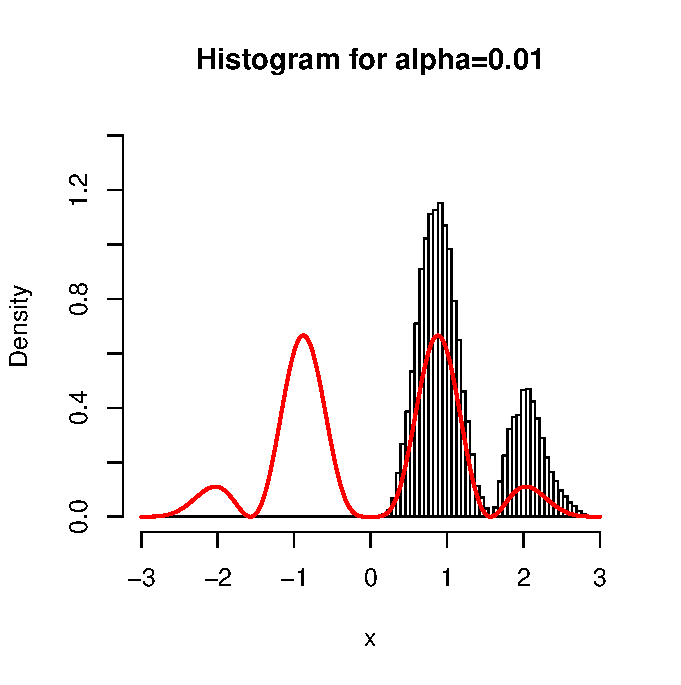
\includegraphics[width=0.4\textwidth]{figures/alpha-small}
	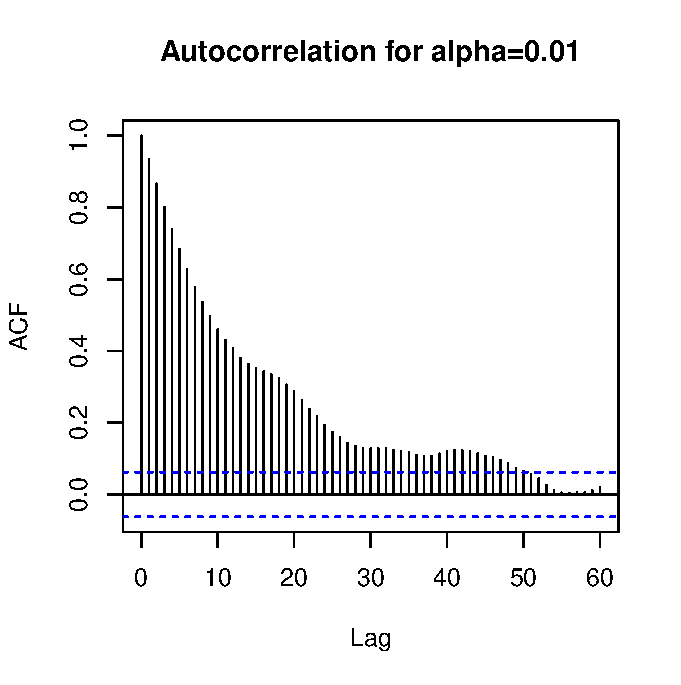
\includegraphics[width=0.4\textwidth]{figures/auto-alpha-small}
	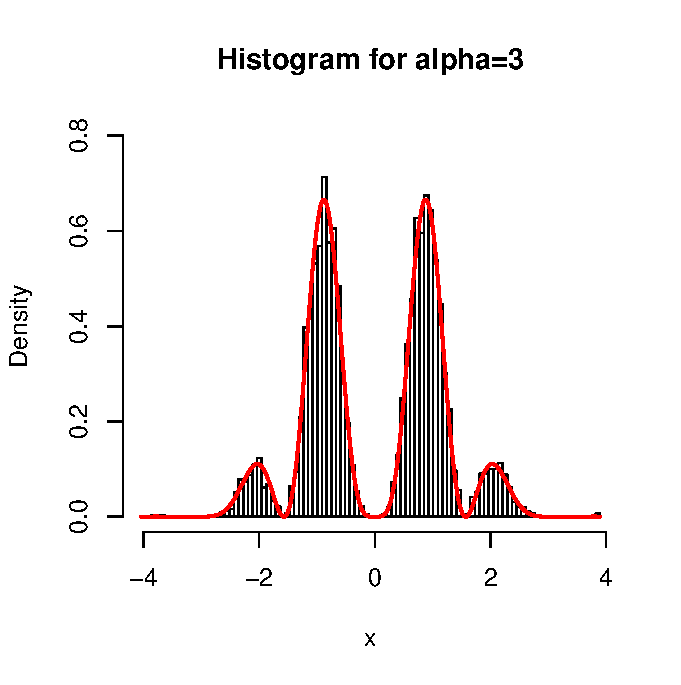
\includegraphics[width=0.4\textwidth]{figures/alpha-optimal}
	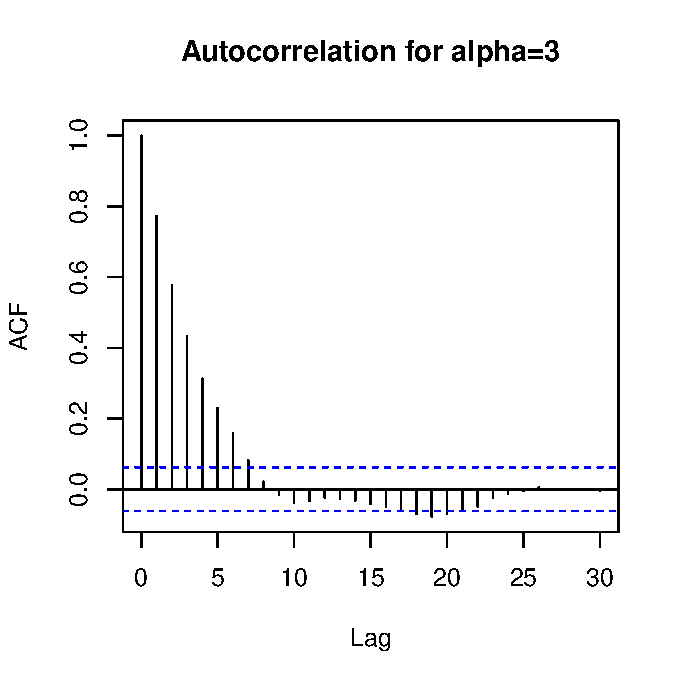
\includegraphics[width=0.4\textwidth]{figures/auto-alpha-optimal}
	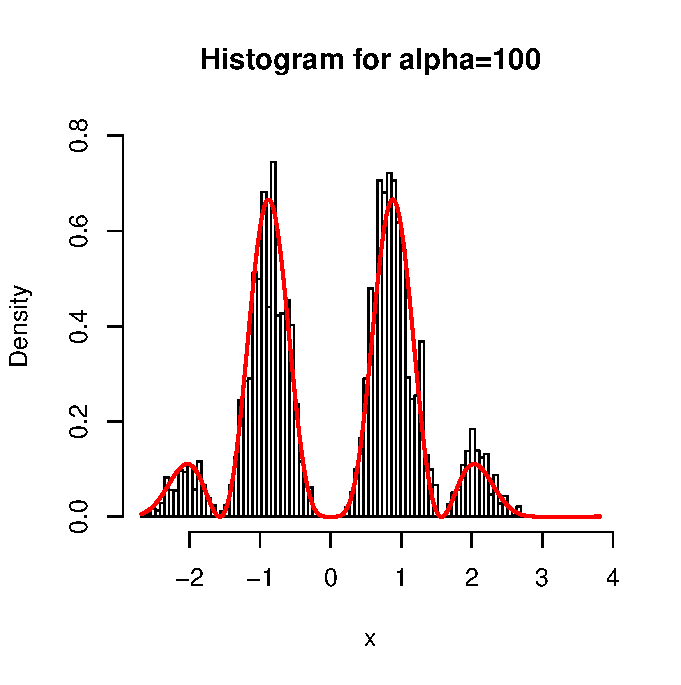
\includegraphics[width=0.4\textwidth]{figures/alpha-big}
	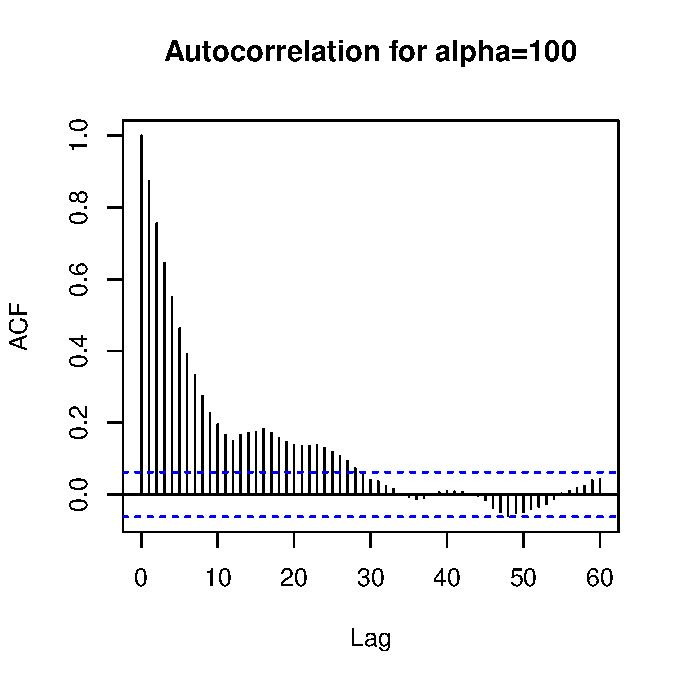
\includegraphics[width=0.4\textwidth]{figures/auto-alpha-big}
%	\tag{1}
	\caption{Histograms and autocorrelation functions of for three different variances \(\alpha\) of the Gaussian proposal distributions. It is apparent that the histogram for \(\alpha=3\) fits the actual density the best and also that the autocorrelation decays the quickest for this parameter. Note that for \(\alpha=0.01\) the MH random walk only explored some area of high density. The actual density if obtained by numerical integration.}
	\label{fig:4.1.2}
\end{figure}

\end{ex}

\begin{emp}[Tuning the proposal]\label{tuning}
In order to obtain a higher acceptance rate without simply choosing the variance of the proposal distribution small one can \emph{tune} or \emph{adapt} the proposal distribution. This means one adjusts the proposal distribution after a while, lets say after the first \(10^3\) samples in such a way that one replaces the original covariance matrix \(\Sigma\) by the empirical covariance of the first \(10^3\) samples%recent\todo{is this true?}
. Then one forgets about all the samples so far -- they are called usually the \emph{burn in period} -- and starts a new MH random walk usually at one of the data points of the burn in period, since they should already indicate where an area of high density is. It is essential to drop the first samples since otherwise the Markov property would break as all further samples now rely on the coveriance of the first burn in period and hence on those points. 
The reason why this increases the acceptance rate is, that the proposal now only is aggressive in those directions where the density is widely spread. For a further discussion we refer to \cite{roberts2009examples}. %recent\todo{find a reference for this}%This effect can be seen in Figure \todo{make this figure}.
\end{emp}

\begin{emp}[The Gelman-Rubin diagnostic]
\todo{!}
\end{emp}

\subsection{Slice sampling}

Slice sampling is a different MCMC method and quite similar to the MH random walk. Nevertheless it has the benefit that one does not have to define a family of proposal distributions and that the constructed Markov chain is always irreducible. However, we will see that at least when one wants to simulate the slice sampling one runs into similar problems of having to choose a parameter that influences the auto correlation function and hence the speed of convergence of the method. We begin by fixing our frame we will work in. %  where one has to model 

\begin{emp}[Setting]
Let \(\Theta\) be a measurable space, \(\mu\) a measure on that space and \(f\colon\mathcal X\to[0, \infty]\) a function with finite integral
\[Z \coloneqq \int\limits_{\mathcal X} f(x) \mu(\mathrm{d}x)\in(0, \infty).\]
In particular there is \(\hat x\in\mathcal X\) such that \(f(\hat x)>0\). Our goal is to find an ergodic Markov chain with invariant distribution
\[\pi(A)\coloneqq \frac1Z \int\limits_A f(x)\mu(\mathrm dx). \]
Further we will assume -- after an eventual modification of \(f\) on a \(\mu\) Null set -- that 
\[f\le \left\lVert f \right\rVert_{L^\infty(\mu)} = \inf \Big\{ \alpha\in\mathbb R \;\big\lvert\; f \le \alpha \text{ almost surely with respect to } \mu \Big\}\in[0, \infty]. \]
\end{emp}

\begin{emp}[The slice sampling method]
Assume we have already given the first \(n\) samples \(x_1, \dots, x_n\) of the Markov chain. If we have \(f(x_n)=0\), then we set \(x_{n+1}\coloneqq \hat x\). Otherwise we sample \(y\) according to the uniform distribution on \([0, f(x_n)]\) and define the \emph{slice}
\[S\coloneqq S(y)\coloneqq \left\{ x\in\mathcal X \mid f(x) \ge y \right\}. \]
\begin{figure}[h!]
	\centering
	\includegraphics[width=0.6\textwidth]{figures/Slice-sampling-neal-new}
%	\tag{1}
	\caption{Schematic sketch of the selection of a slice: (a) first \(y\) is sampled uniformly in \([0, f(x_0)]\) and (b) the slice is selected. Original graphic from \cite{neal2003slice}.}
	\label{fig:4.2}
\end{figure}

Note that because \(y < f(x_n)\le \left\lVert f \right\rVert_{L^\infty(\mu)}\) holds almost surely, we have \(\mu(S)>0\) as well as
\[ \mu(S) \le y^{-1} \int\limits_S f(x)\mu(\mathrm dx)<\infty \]
where we used Markov�s inequality as well as \(y>0\) almost surely. Now draw \(x_{n+1}\) according to the uniform distribution\footnote{Of course we mean the uniform distribution with respect to \(\mu\) that gives weight \(\mu(S)^{-1} \cdot \mu(A)\) to a set \(A\subseteq S\).} on \(S\). Note that \(f(x_n)>0\), then \(f(x_{n+1})\ge y > 0\) almost surely, hence \(f(x_n) = 0\) can only hold for \(n=0\). Further the reason why we have to treat the case \(f(x_n)=0\) individually is, that there typically is no uniform distribution on the slice \(S(0) = \mathcal X\).
In pseudo code the steps of the resulting Markov chain can be written in the following form.
\begin{algorithm}
\caption{A single slice sampling step \label{alg:slice-sampling}}
\begin{algorithmic}[1]
\Require{Current state \(x_n\) of the Markov chain}
 \If \(f(x_n) = 0\)
  \State \(x_{n+1}\gets \hat x\)
\Else
  \State \(y\sim \mathcal U([0, f(x_n)])\)
  \State \(S\gets \left\{ x\in\mathcal X \mid f(x) \ge y \right\}\)
  \State \(x_{n+1} \sim \mathcal U(S)\)
\EndIf
\State\Return{\(x_{n+1}\)}
\end{algorithmic}
\end{algorithm}
\end{emp}
%\todo{maybe add a picture?}

%\Require{First \(n\) samples \(x_1, \dots, x_n\)}
%\If{\(f(x_n) = 0\)}
%  \State \(x_{n+1}\gets x_0\)
  %\Break
%\Else
%  \State \(y\sim \mathcal U([0, f(x_n)])\)
%  \State \(S\gets \left\{ x\in\mathcal X \mid f(x) \ge y \right\}\)
%  \State \(x_{n+1} \sim \mathcal U(S)\)

If we compare the Markov chain to the MH random walk, we notice that in the slice sampling we first create a random threshold \(y\) and then sample uniformly from all points that satisfy this threshold. This is just the other way round than in the MH random walk where we first make a proposal for the next state of the Markov chain and then decide whether we will accept it or not.

Just like in the case of the MH random walk we can explicitly give the transition kernel and use this expression then to check that \(\pi\) is a stationary distribution. The kernel of the Markov chain that arises from the slice sampling iteration is given by
\begin{equation*}
\begin{split}
K(x, A) & = \int\limits_\mathbb R\frac{\mathds{1}_{[0, f(x)]}(y)}{f(x)} \cdot \frac{\mu(A\cap S(y))}{\mu(S(y))} \lambda(\mathrm dy) \\
& = \int\limits_\mathbb R\frac{\mathds{1}_{[0, f(x)]}(y)}{f(x)} \cdot Z(y)^{-1} \int\limits_A \mathds{1}_{[y, \infty)}(f(z)) \mu(\mathrm dz) \lambda(\mathrm dy)
\end{split}
\end{equation*}
where \(\lambda\) is the Lebesgue measure on \(\mathbb R\), \(\mathds{1}\) is the indicator function and \(Z(y)\) is the normalisation constant
\[Z(y)\coloneqq \int\limits_{\mathcal X} \mathds{1}_{[y, \infty)}(f(z)) \mu(\mathrm dz) = \mu(S(y)) \in(0, \infty). \]
Obviously the expression above only holds if \(f(x)>0\) and in the case \(f(x) = 0\) we have
\[K(x, A) = \delta_{\hat x}(A).\]

\begin{prop}[Invariant distribution]
The probability distribution \(\pi\) is a stationary distribution of the Markov chain associated with the slice sampling method.
\end{prop}
\begin{proof}
For any \(A\subseteq\mathcal X\) we can compute
\begin{equation*}
\begin{split}
\int\limits_{\mathcal X} K(x, A) \pi(\mathrm dx) & = \frac1Z\int\limits_{\mathcal X }\int\limits_\mathbb R\frac{\mathds{1}_{[0, f(x)]}(y)}{f(x)}\cdot Z(y)^{-1} \int\limits_A \mathds{1}_{[y, \infty)}(f(z)) \mu(\mathrm dz) \lambda(\mathrm dy) f(x) \mu(\mathrm dx) \\
& =\frac1Z \int\limits_{ A }\int\limits_\mathbb R Z(y)^{-1} \int\limits_{\mathcal X}\mathds{1}_{[y, \infty)}(f(x)) \mu(\mathrm dx) \mathds{1}_{[0, f(z)]}(y) \lambda(\mathrm dy) \mu(\mathrm dz) \\
& = \frac1Z\int\limits_A f(z)\mu(\mathrm dz) = \pi(A)
\end{split}
\end{equation*}
where we again used Fubini�s theorem for non negative functions.
\end{proof}

\begin{prop}[Irreducibility]
The Markov chain that arises from the slice sampling algorithm is \(\pi\) irreducible.
\end{prop}
\begin{proof}
Fix \(A\subseteq\mathcal X\) with positive probability \(\pi(A)>0\) and \(x\in\mathcal X\). If we have \(f(x)>0\), then we have \(\mu(A\cap S(y))>0\) for one \(y\in(0, f(x))\). We obtain
\[K(x, A) \ge \int\limits_{\mathbb R} \frac{\mathds{1}_{[0, y]}(z)}{f(x)} \cdot \frac{\mu(A\cap S(z))}{\mu(S(z))} %\frac{y}{f(x)}\cdot \frac{\mu(A\cap S(y))}{\mu(S(0))} 
> 0. \]
If however \(f(x)=0\), then we get
\[K^2(x, A) = K(\hat x, A) > 0. \]
\end{proof}

\begin{theo}[Ergodicity]
%Assume that the unnormalised density admits the factorisation \(f(x) = q(x)l(x)\) where \(q\) and \(l\) are measurable and \(l\) is non negative. 
If \(f\) is bounded, the Markov chain induced by the slice sampling method is ergodic.
\end{theo}
\begin{proof}
See Theorem 6 in \cite{mira2002efficiency}.
\end{proof}

%Under the condition of the theorem above one even obtains a stronger version of ergodicity, namely uniform %in the starting point \(\)
%\[\sup_{x\in\mathcal X} \left\lVert \hat{\mathbb P}_n - \pi \right\rVert_{TV} \xlongrightarrow{n\to\infty} 0. \]

%recent\todo{Let someone check whether this is correct...}

\subsubsection*{Implementation details}

Just like in the case of the MH random walk we will provide a few comments about the actual simulation of the slice sampling algorithm %Again those will rather be general guide lines and not be justified by rigorous arguments.
and for this, we will assume \(\mathcal X\subseteq\mathbb R^d\).

The main difficulty in the implementation is the sampling of a uniform distribution on a slice \(S\). In practice it is not even possible to calculate the slice but one can exploit the %and therefore one has to come up with a trick. This trick is based on the
following observation. Assume that we are able to simulate a uniform distribution on a set \(C\) that contains the slice \(S\). Then the following algorithm -- which is nothing but the conditioning of this uniform distribution on the event that the outcome is in \(S\) -- samples uniformly from \(S\).
\begin{algorithm}
\caption{Sampling from a uniform distribution on a subset \(S\subseteq C\) \label{alg:slice-sample}}
\begin{algorithmic}[1]
\Require{\(S\) and \(C\supseteq S\)}
\State \(x\sim\mathcal U(C)\)
\While {\(x\notin S\)}
  \State \(x\sim\mathcal U(C)\)
\EndWhile
\State\Return{\(x\)}
\end{algorithmic}
\end{algorithm}

An obvious choice for \(C\) would be a cuboid 
\[C = \prod_{i = 1}^d [a_i, b_i]\]
since it is straight forward to sample from a uniform distribution on a cuboid. Namely one only has to sample the individual coordinates uniformly in the intervals \([a_i, b_i]\). The problem still remains how one can find a cuboid that surely contains the whole slice \(S\). The short answer is that there is no general way to do this. However, not everything is lost, since we can use random cuboids that have the property that every part of the slice is contained in the cuboid with positive probability. This will be crucial in retaining the irreducibility of the Markov chain. In fact it has been found that in applications the following procedure works well%recent\todo{cite}
. Given the current state \(x_n\) of the Markov chain, we propose a random interval \([a_i, b_i]\) around the \(i\)-th component fo \(x_n\). Then we extend those intervals until the endpoints \(a\) and \(b\) of the cuboid do not lie in the slice anymore which is described in Algorithm \ref{alg:cuboid}.  %Further the algorithm returns the 
\begin{algorithm}
\caption{Sampling a random cuboid \label{alg:cuboid}}
\begin{algorithmic}[1]
\Require{Current state \(x_n\) of the Markov chain, parameter \(\alpha>0\)}
\For {\(i=1, \dots, d\)}
  \State \(a_i, b_i \sim \mathcal E(\alpha)\)
%  \State \(b_i \sim \mathcal E(\alpha)\)
\EndFor
\State \(a\gets (a_1, \dots, a_d), b\gets(b_1, \dots, b_d)\)
\While {\(x - a \in S\)}
  \State \(a \gets 2 \cdot a\)
\EndWhile
\While {\(x + b \in S\)}
  \State \(b \gets 2 \cdot b\)
\EndWhile
\State\Return{\((x - a, x + b)\)}
\end{algorithmic}
\end{algorithm}

Here \(\mathcal E(\alpha)\) denotes the exponential distribution with parameter \(\alpha\) and determines how large the first proposed intervals are. Note that it is straight forward and computationally very easy to determine whether a point \(x\) is in the slice \(S(y)\) since one only has to check \(f(x) \ge y\). The reason for the choice of the exponential distribution is that this ensures that the cuboid can get arbitrarily large with positive probability. This leads to the effect that the Markov chain one obtains in exchanging the sample from \(\mathcal U(S)\) by a sample from \(\mathcal U(S\cap C)\) still is irreducible. %\todo{explain this in greater detail}.
To see this we can slightly modify the proof of irreducibility, so for \(A\subseteq\mathcal X\) with positive probability we choose \(y>0\) such that \(\mu(A\cap S(y))>0\). Further we can choose a cuboid \(C\) around \(x\) such that \(\mu\big(A\cap S(y)\cap C\big)>0\). Further this cuboid is contained in the cuboid proposed by Algorithm \ref{alg:cuboid} with positive probability and hence we have
\[K(x, A) = \mathbb P_x(X_1\in A) %\ge \frac{y}{f(x)} \cdot \delta \cdot \frac{\mu\big(A\cap S(y)\cap C\big)}{\mu(S(y)\cap C)} 
> 0. \]

Finally we can present the pseudocode of the algorithm that arises from the combination of the usual slice sampling method and the approximation of the uniform distribution on the slice.

\begin{algorithm}
\caption{Algorithm for the slice sampling \label{alg:slice-sampling-implementation}}
\begin{algorithmic}[1]
\Require{Unnormalised density \(f\), starting value \(x_0\), desired length \(n\) of the chain, \(\alpha>0\)}
\If {\(f(x_0) = 0\)}
  \State \(x_0 \gets \hat x\)
\EndIf
\For {\(i = 0, \dots, n-1\)}
  \State \(y\sim \mathcal U([0, f(x_{i})])\)
  \State \(C\) random cuboid around \(x_{i}\) with parameter \(\alpha\)
  \State \(x\sim\mathcal U(C)\)
  \While {\(f(x)<y\)}
    \State \(x\sim\mathcal U(C)\)
  \EndWhile
  \State \(x_{i+1} \gets x\)
\EndFor
\State\Return{\(x = (x_0, \dots, x_n)\)}
\end{algorithmic}
\end{algorithm}

It shall be noted, that the above algorithm also uses a point \(\hat x\) of positive density, which can be determined easily for a lot of densities \(f\). If this is however not straight forward, one could also sample \(x_0\) according to a normal distribution until we select a point of positive density.

Obviously the algorithm presented above produces a Markov chain that is not identical with the one presented in the theoretical discussion of the slice sampling method. However, if one wants to ensure the convergence of this slightly modified Markov chain, one has to check whether \(\pi\) remains a stationary distribution and whether the chain is still ergodic. This is usually done in the specific setting one works in, cf. \cite{neal2003slice}. We will quickly discuss this in a very easy case. Namely let us assume \(d=1\) and that \(f\) is continuous and has only one local maximum. We call \(f\) \emph{unimodal} in this case and note that every slice \(S(y)\) is an interval. Hence, the proposed cuboid is an interval around \(x_n\in S(y)\) such that both endpoints are outside of the slice \(S(y)\) and hence we have \(S(y)\subseteq C\). Therefore, the algorithm above is equivalent to the original slice sampling method and hence produces an ergodic Markov chain with the desired invariant distribution.
%Further we will quickly discuss the case where \(f\) has only one local maximum and we call \(f\) \emph{unimodal} in this particular case.

\begin{emp}[The choice of \(\alpha\)]
One could think that a small choice of \(\alpha\) -- which relates into large values of \(a_i\) and \(b_i\) -- would be the best since this increases the probability that the whole slice \(S\) is contained in the cuboid \(C\). There is some truth in this approach, since \(\mathcal U(S\cap C)\) is a better approximation of \(\mathcal U(S)\) if \(C\) is larger and further the while loops in Algorithm \ref{alg:cuboid} need less repetitions if \(a_i\) and \(b_i\) initially are big. This relates into longer running time of the algorithm that samples the random cuboid. However, one should not choose \(\alpha\) too small, because a large cuboid \(C\) also means that a lot of samples from \(\mathcal U(C)\) will lie outside of \(S\cap C\). Hence, Algorithm \ref{alg:slice-sample} that samples from \(\mathcal U(S\cap C)\) will get slower as it will need more repetitions of the while loop.

In conclusion there is a trade off in terms of computation time between the choice of too small and too large values for \(\alpha\). %This choice effects the decay of the auto correlation and the effective sample size just like in the case of the MH random walk.
However not always the parameter \(\alpha\) that minimises the simulation time is the most suitable, since the autocorrelation decreases together with the parameter \(\alpha\). % like it can be seen in Figure \ref{fig:4.3}.
 Hence computation time should rather be compared to the effective sample size.% For an %However since the computation time increases for small \(\alpha\)  This can be seen in Figure\todo{make figure}.

Those effects of \(\alpha\) on the auto correlation and therefore effective sample can be seen in Figure \ref{fig:4.3} where the procedure of Example \ref{example} is repeated but this time with the slice sampling method. The sample size remains \(2\cdot10^4\) and the different parameter choices where \(\alpha = 0.01, 0.5, 10\). The according computation times where approximately \(26\si{s}\) for \(\alpha=0.01\), \(1.7\si{s}\) for \(\alpha=0.5\) and \(1.7\si{s}\) for \(\alpha=10\). In regard of the decay of the autocorrelation functions and the resulting effective sample sizes, it is apparent that the choice \(\alpha = 0.5\) would be the most sensible one in this case.

\begin{figure}[h!]
	\centering
	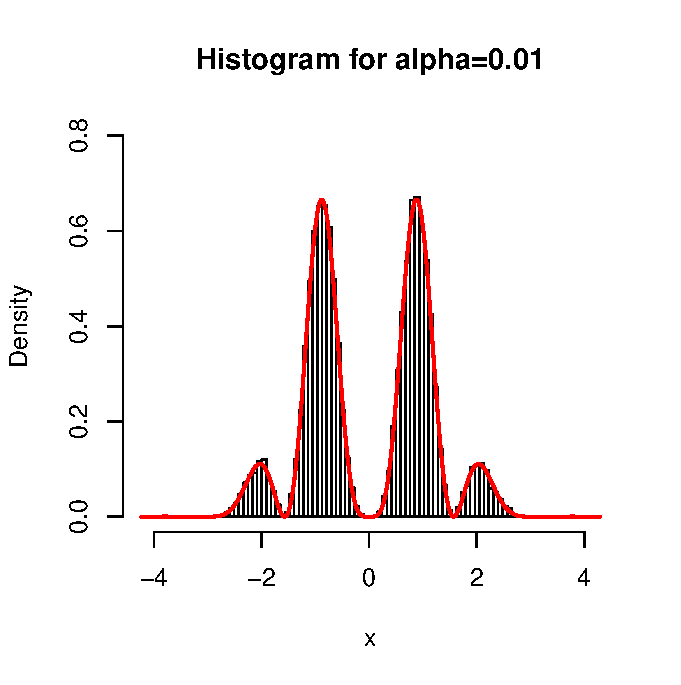
\includegraphics[width=0.42\textwidth]{figures/slice-alpha-small}
	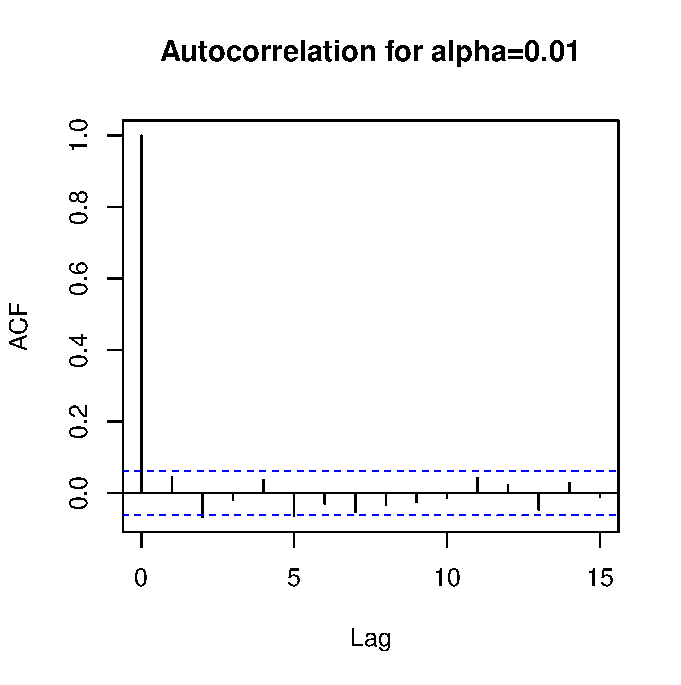
\includegraphics[width=0.42\textwidth]{figures/slice-auto-alpha-small}
	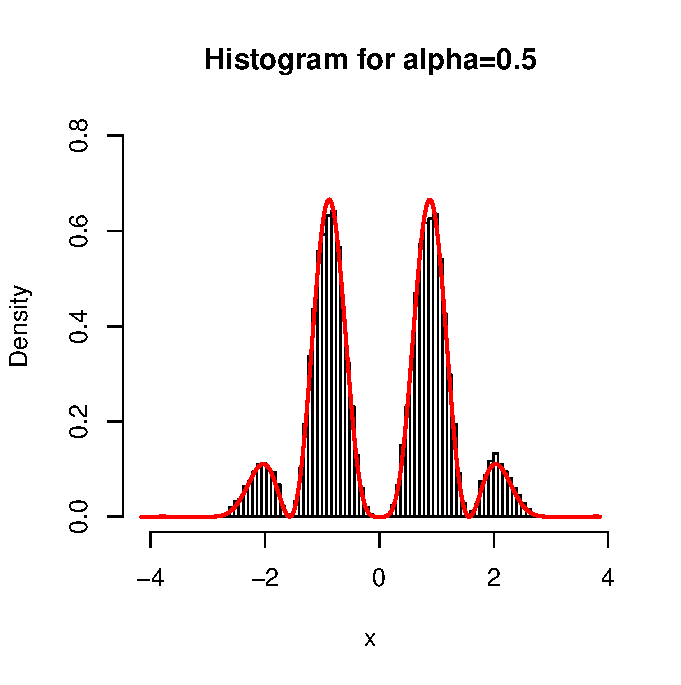
\includegraphics[width=0.42\textwidth]{figures/slice-alpha-optimal}
	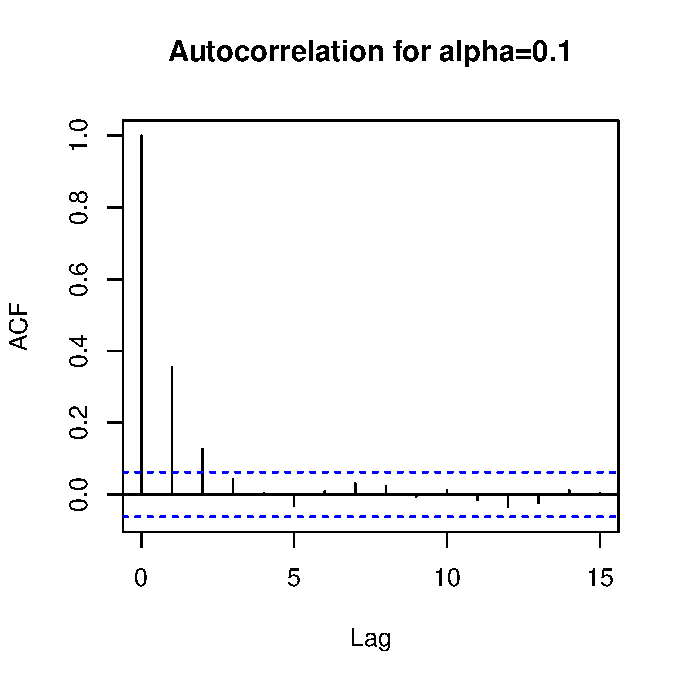
\includegraphics[width=0.42\textwidth]{figures/slice-auto-alpha-optimal}
	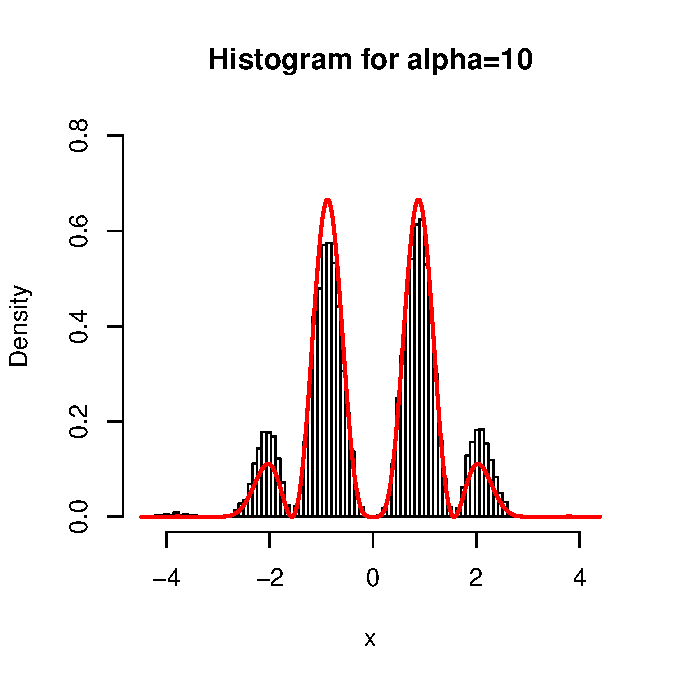
\includegraphics[width=0.42\textwidth]{figures/slice-alpha-big}
	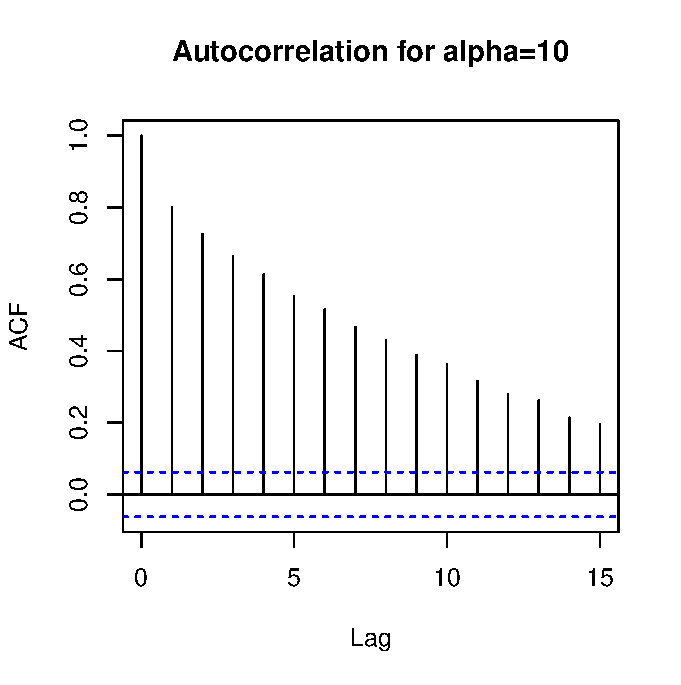
\includegraphics[width=0.42\textwidth]{figures/slice-auto-alpha-big}
%	\tag{1}
	\caption{Histograms and autocorrelation functions for the choices of \(\alpha = 0.01, 0.5, 10\). The auto correlation obviously decreases the fastest for \(\alpha=0.01\), however the computation time is much higher than for the parameter the other parameters.}
	\label{fig:4.3}
\end{figure}
\end{emp}

%\subsection{Tuning the algorithm}
%\todo{add remark what happens if the integral is not finite}

\subsection{Variational MCMC methods}

Now that we have presented a general setup for MCMC methods we wish to use them to approximated the posterior distribution which is given by the unnormalised density %is given in unnormalised form %given by \eqref{post2}
\begin{equation}\label{post3}
f(\theta) = f_\Theta(\theta) \prod_{i=1}^n \frac{\det(L(\theta)_{A_i})}{\det(L(\theta) + I)}.
\end{equation}
In the light of the theoretical guarantees this will surely work and actually Figure \ref{fig:4.1} has been created this way. However, the evaluation of this unnormalised density \(f\) can take several seconds or even minutes itself since it involves the computation of the determinant of the \(N\times N\) matrix \(L(\theta) + I\). %is the computational bottle neck of this procedure and leads to long computation times. This is due to the calculation of the \(N\times N\) determinant \(\det(L(\theta) + I)\).
However, one can efficiently compute bounds of the unnormalised density and we will provide a general setup of how the MH random walk and slice sampling can be expressed using those bounds. This will lead to significatnly shorter simulation times for the respective MCMC methods. % such bounds can be used to obtain a

\begin{emp}[Setting]
Let \(\Theta\) be a measurable space, \(\mu\) a measure on that space and \(f\colon\mathcal X\to[0, \infty]\) a function with finite positive integral
\[Z = \int\limits_{\mathcal X} f(x) \mu(\mathrm{d}x)\in(0, \infty).\]
Let further \(f\le \left\lVert f \right\rVert_{L^\infty(\mu)}\) and let
\[\left\{ f(\cdot|x) \mid x \in\mathcal X\right\}\]
be a family of proposel distributions.
Let now \(f_n^-, f_n^+\colon\mathcal X\to [0, \infty]\) be functions such that \(f_n^-(x)\le f(x)\le f_n^+(x)\) for all \(x\in\mathcal X\) as well as
\[f_n^\pm(x) \xlongrightarrow{n\to\infty} f(x) %\quad \text{and } f_n^+(x)\to f(x) \quad \text{for } n\to\infty 
\quad \text{for all } x\in\mathcal X. \]
We seek an expression of the MH random walk and the slice sampling method that purely relies on those bounds \(f_n^-\) and \(f_n^+\) of the unnormalised density.
\end{emp}

\subsubsection*{Variational MH random walk}

We note that the only part in the algorithm for the MH random walk where \(f\) is needed itself is the accept-reject step, hence, it suffices to adjust this step. % to purely rely on the bounds \(f_n^\pm\).
In order to achieve this we bound the acceptance rate through
\[\rho_n^\pm(x, y) \coloneqq \min\left\{ \frac{f_n^\pm(y) f(x|y)}{f_n^\mp(x)f(y|x)}, 1\right\}.\]
In fact we obviously have \(\rho_n^-(x, y)\le\rho(x, y)\le\rho_n^+(x, y)\) as well as
\[\rho_n^\pm(x, y)\xlongrightarrow{n\to\infty}\rho(x, y) \quad\text{for all } x, y\in\mathcal X. \]
Hence if we want to decide whether a number \(a\) satisfies \(a\le \rho(x, y)\) we can iteratively tighten the upper and lower bounds on \(\rho\) until we either have \(a\le\rho_n^-(x, y)\) and thus \(a\le\rho(x, y)\) or \(a>\rho_n^+(x, y)\) and therefore \(a>\rho(x, y)\).
Now we can adjust the algorithm of the MH random walk accordingly and obtain Algorithm \ref{alg:variational-MH}.

\begin{algorithm}
\caption{One step in the variational MH random walk \label{alg:variational-MH}}
\begin{algorithmic}[1]
\Require{Current state \(x_n\) of the MH random walk}
\State \(y\sim f(\cdot|x_n)\mathrm d\mu\)
\State \(a\sim \mathcal U([0, 1])\)
\State \(k\gets 1\)
\While {\(a>\rho_k^-(x_n, y)\) and \(a\le \rho_k^+(x_n, y)\)}
  \State \(k \gets k+1\)
\EndWhile
\If{\(a\le \rho_k^-(x_n, y)\)}
  \State \(x_{n+1}\gets y\)
\Else 
  \State \(x_{n+1}\gets x_n\)
\EndIf
\State\Return{\(x_{n+1}\)}
\end{algorithmic}
\end{algorithm}

\subsubsection*{Variational slice sampling}

In the slice sampling we use the unnormalised density twice. The first time by sampling \(y\sim\mathcal U([0, f(x_n)])\) and the second time when checking \(x\in S(y)\) or equivalently \(f(x)\ge y\). For the first problem we note that we surely have \([0, f(x_n)]\subseteq [0, f_1^+(x_n)]\) and hence we can use Algorithm \ref{alg:slice-sample} to sample uniformly from \([0, f(x_n)]\). However, in this algorithm we need to check \(y\in [0,f(x_n)]\) or equivalently \(f(x_n)\ge y\) which is just what we had to do determine whether \(x\in S(y)\). Therefore, it suffices to see how one can check \(f(x)\ge y\) which we will do analogously to the variational MH random walk by gradually tightening the bounds. This yields Algorithm \ref{alg:decide} that returns �TRUE� if \(f(x)\ge y\) and �FALSE� otherwise.

\begin{algorithm}
\caption{Deciding \(f(x)\ge y\) through the bounds \label{alg:decide}}
\begin{algorithmic}[1]
\Require{\(y\in\mathbb R\) and \(x\in\mathcal X\)}
\State \(k\gets 1\)
\While {\(y>f_k^-(x)\) and \(y\le f_k^+(x)\)}
  \State \(k \gets k+1\)
\EndWhile
\If{\(y\le f_k^-(x_n, y)\)}
  \State \Return{TRUE}
\Else 
  \State \Return{FALSE}
\EndIf
\end{algorithmic}
\end{algorithm}

In conclusion we can express both MCMC methods exactly through those bounds as long as the bounds converge. This enables a fast simulation of the Markov chains if the unnormalised density is slow the bounds \(f_n^\pm\) are easy to compute. In the case that \(f\) is the posterior \eqref{post3} of a DPP such bounds are given in \cite{affandi2014learning} and \cite{bardenet2015inference}.
%this decision algorithm in combination with Algorithm \ref{alg:slice-sample} gives an expression of the slice sampling Markov chain completely through the bounds \(f_n^\pm\).

\chapter{Toy example: Learning the log linearity constant of a spatial DPP}

We will apply the MLE and the Bayesian estimation for one log linear model in a controlled environment, i.e. where the data is generated by ourselves. This will clearly show how the Bayesian approach allow to encode more information. Further we will see how the regulariser or prior affects the estimation and will quickly discuss how this impacts the noise sensitivity of the estimation.

We continue the example of the DPP on a two dimensional grid in the unit square from the first chapter. For this we note that for a \(100\times100\) grid the evaluation of the elementary probabilities 
\[ f(A|\theta) = \frac{\det(L(\theta)_A)}{\det(L(\theta) + I)} \]
would involve the calculation of a determinant of a \(10^4\times 10^4\) matrix and even the storage of such a matrix would pose a problem since it consists of \(10^8\) numbers. If the storage of a real number is done in the double-precision floating-point format, it takes \(64\) per number and the space required to store the entire matrix is \(64\times 10^8\si{bit} = 800\si{MB}\), so almost one Gigabyte.\footnote{One byte is defined to be \(8\) bits. The units of Megabytes and Gigabytes are defined in the familiar way and denoted by \(\si{MB}\) and \(\si{GB}\) respectively.} This makes even the computation of the log likelihood function very time consuming, let alone its maximisation. Because of those computational hindrances we will decrease the size %of the grid to \(30\times30\)
%for computational reasons,
 but the ideas remain exactly the same.
%We will recall the definition of the model and also give the exact values of the parameters chosen.

\begin{emp}[Setting]
We set
\[\mathcal Y \coloneqq 39^{-1} \left\{ 0, \dots, 39\right\}^2 \]%\left\{ (i, j) \mid 39\cdot  \right\} \]
and obtain a \(40\times 40\) grid in the unit square. We again choose \(\mathcal R \coloneqq \mathcal Y \) and \(f\) to be %the normal density with mean \(0\) and variance \(10>0\). Then we choose the similarity feature vectors to be 
\[f(x) \coloneqq \exp\left( - 8\cdot x^2\right) \]
and set
\[(\phi_i)_j\propto f(\left\lVert i - j \right\rVert) \quad \text{for } i, j\in\mathcal Y.\]
Further we choose the qualities to be be decreasing with the distance from the centre \(m\) of the and set
\[q_i\coloneqq e^6 \cdot \exp\big(-10 \left\lVert i - m \right\rVert\big) = \exp\big( - 10\left\lVert i - m \right\rVert + 6\big). \]
\end{emp}

%The exact constants in the function \(f\) and the qualities \(q_i\) where adjusted so that the repellent property of the DPP is visible, a drop off of the qualities towards the corners is visible and a reasonable cardinality of the DPP is obtained. 
The goal is to estimate the two parameters that characterise the qualities, which are \(e^6\) and \(-10\). In order to do this we note that the qualities are given by a log linear model since we have
\[q_i = \exp(\theta_0^Tf_i) \quad \text{where } f_i = \begin{pmatrix}
\left\lVert i - m \right\rVert \\ 1
\end{pmatrix} \text{ and } \theta_0 = \begin{pmatrix}
-10 \\ 6
\end{pmatrix}.\]

Hence we should be able to estimate this log linearity constant \(\theta\in\mathbb R^2\) based on some data that is distributed according to this DPP. To do this we generate \(n=20\) samples \(A_1, \dots, A_n\) from the DPP using the sampling algorithm introduced in the first chapter. % and define the log likelihood function associated with those observations and the actual similarity kernel \(S_{ij} = \phi_i^T\phi_j\).

\section{MLE and regularised MLE}

In order to perform the maximum likelihood estimation for the log linearity constant, we need to fix a similarity kernel \(\hat S\), but since we know the exact kernel, we can simply set \(\hat S_{ij} \coloneqq \phi_i^T\phi_j\). Then we maximise the log likelihood over \(\mathbb R^2\) using a pre-implemented optimisation algorithm in R. The resulting estimate was
\begin{equation}\label{mletheta}
\hat\theta = \begin{pmatrix}
-10.000250 \\ 6.007382
\end{pmatrix}
\end{equation}
but from the consistency results we already knew that it should get close to the actual parameter for large sample sizes. Since we also want to investigate the effect of a regulariser, we define two different regularisers
\[F_1(\theta)\coloneqq -\frac{\left\lVert \theta \right\rVert^2}{2^4} \quad \text{and } F_1(\theta)\coloneqq -\frac{\left\lVert \theta \right\rVert^2}{2} \]
as a regulariser. Note that those corresponds to the priors
\begin{equation}\label{toyprior}
f_{\Theta_1}(\theta) = \exp\left(-\frac{\left\lVert \theta \right\rVert^2}{2^4}\right) \quad \text{and } f_{\Theta_2}(\theta) = \exp\left(-\frac{\left\lVert \theta \right\rVert^2}{2}\right)
\end{equation}
which are Gaussian priors with different variance. Under those regularisations, the respective MAPs obtained were
\[\hat\theta_1 = \begin{pmatrix}
-9.870850 \\ 5.952101
\end{pmatrix} \quad \text{and } \hat\theta_1 = \begin{pmatrix}
-9.050763 \\ 5.597739
\end{pmatrix}.\]
It is not surprising that regularised MLEs are closer to zero, since the regulariser is built to penalise large parameter values. Further the effect of the Gaussian prior with smaller variance -- which is the second one -- is larger, which is consistent with the heuristic explanation that it cooperates a stronger prior believe, since it predicts that the parameter is more likely to be close to zero.

We chose the sample size of \(n=20\) relatively small and want to show the effect the sample size has on the estimation. Obviously, we know from the second chapter that the MLE will converge to the actual parameter. To show this convergence in our case, we iteratively raised the sample size from \(1\) to \(30\) and obtained the maximum likelihood estimators that are shown in Figure \ref{fig:learningcurve}. We can see that the MLE converges towards the actual parameter \todo{rewrite this!}
where the regularised MLE seems to converge to a very similar value where the difference of the limits is smaller than the fluctuations. Nevertheless we will see in the comments on the model selection that the Bayes factor between the two models is very high and hence the unregularised model is favourable. \todo{check this}%This is because the regularisation is not very strong in this case and we will see later that the models are actually quite close together meaning that the Bayes factor is not very high.% \todo{check this} % \todo{does this mean the effect of the regularisation vanishes?}
\begin{figure}[h!]
	\centering
	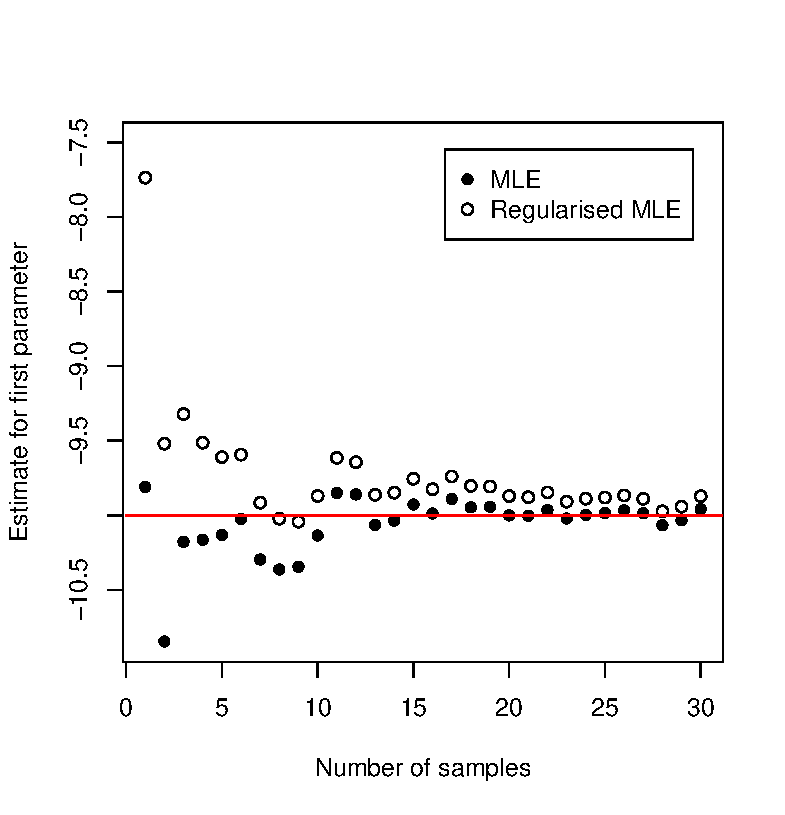
\includegraphics[width=0.49\textwidth]{figures/Learning-curve-comparison-first-parameter}
	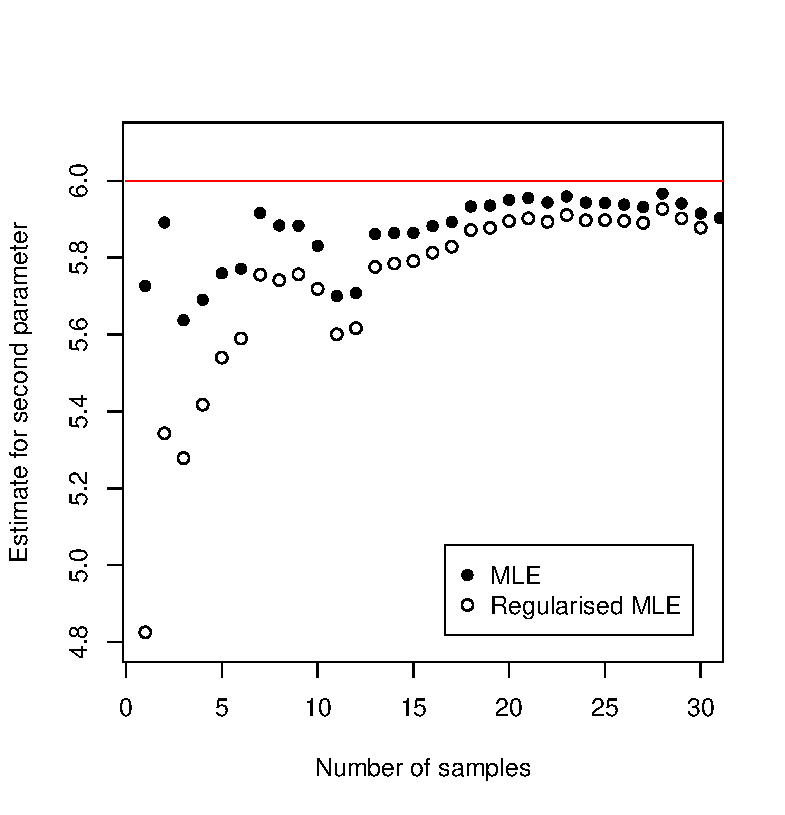
\includegraphics[width=0.49\textwidth]{figures/Learning-curve-comparison-second-parameter}
%	\tag{1}
	\caption{Plot of the progression of the MLE and regularised MLE. The real parameter is marked by the red lines and with increased sample size they both estimators are within a reasonably small margin.}
	\label{fig:learningcurve}
\end{figure}



\section{Bayesian estimation using MCMC methods}

%We will continue the example of the estimation of the log linearity constant from the section about maximum likelihood estimation and will see how two different priors influence the posterior of the parameter, but first we quickly recall the example.

%\begin{emp}[Setting]
%We work with the \(30\times30\) grid
%\[\mathcal Y \coloneqq 29^{-1} \left\{ 0, \dots, 29\right\}^2 .\]%\left\{ (i, j) \mid 39\cdot  \right\} \]
%Further we set %\(\mathcal R \coloneqq \mathcal Y \) and
% \(f\) to be %the normal density with mean \(0\) and variance \(10>0\). Then we choose the similarity feature vectors to be 
%\(f(x) \coloneqq \exp( - 8\cdot x^2) \) 
%and set
%\[(\phi_i)_j\propto f(\left\lVert i - j \right\rVert) \quad \text{for } i, j\in\mathcal Y.\]
%Finally we choose the qualities to be be decreasing with the distance from the centre \(m\) of the and set
%\[q_i\coloneqq e^6 \cdot \exp\big(-10 \left\lVert i - m \right\rVert\big) = \exp\big( - 10\left\lVert i - m \right\rVert + 6\big). \]
%\end{emp}

We will use the same data set consisting of \(8\) samples from this DPP like in the maximum likelihood estimation and will use the prior \eqref{toyprior}, since it corresponds to the regularised MLE. %that lead to the estimation
%\[\hat\theta = \begin{pmatrix}
%-10.32045 \\   6.07648
%\end{pmatrix}.\]
The posterior of the log linearity parameter is given by
\[f(\theta|A_1, \dots, A_n) \propto f_\Theta(\theta) \prod_{i=1}^n \frac{\det(L(\theta)_{A_i})}{\det(L(\theta) + I)}.\]
%Before we will use the MCMC methods presented
and we will use the MH random walk to approximate it. % In fact this is even easier in practice since one does not have to tune the proposals distributions.
%To do this we will impose a very conservative prior in the sense that we assume to not know the rough size of the parameter theta. Therefore, we define the prior to be a very flat normal distribution centered at the origin and with covariance \(2^{19}\cdot I\). This amounts to almost choosing a uniform distribution on the space and hence we expect to get a similar picture to Figure \ref{fig:4.1}. 
But before we do this, we will shortly discuss how the Bayes factor can be used to decide between two different priors if one has not access to the unregularised and regularised MLE like we did before.

\subsubsection{Comparing different priors via the Bayes factor}

We have introduced the Bayes factor as the ratio of the total observation probabilities under two models. In order to compare 
%the regularised and unregularised model, we need to approximate the total observation probability
\[f(x|\mathcal F) \coloneqq \int_{\Theta} f_{X, \Theta}(x, \theta)\nu(\mathrm{d}\theta)\]
which we will do numerically. 
%Also we have to use normalised priors which means we can not use the generalised constant prior, we have used in the discussion for the Bayesian approach without a prior. Therefore we will work with a uniform distribution on a cuboid and choose it so large that it contains the whole Markov chain by far\todo{What does this mean?}{ }, in our case we choose it to be \([-11, -9]\times[5, 7]\). The Bayes factor obtained by this numerical integration is
%\[24584.31 \approx 2.5\cdot10^4. \]
%This strongly suggests that the model arising from the prior \(f_\Theta\propto \mathds{1}_{[-11, -9]\times[5, 7]}\) is far better suited than the one with the Gaussian prior \eqref{toyprior}.
\todo{Is this not very arbitrary?}

\subsubsection{MCMC simulations}

We proceed in the following steps.

\begin{emp}[First burn in to find a starting point]
%In the first phase we pick the origin as a starting point and choose the proposal \(f(\cdot| \theta)\) to be a Gaussian centered at \(\theta\) and with variance adjust so that an acceptance rate of roughly \(25\%-75\%\) is obtained. Usually if one is starting of at a point in a region with very low density, the variance one has to choose will be rather high.

%This amounts to saying one is very coarsely exploring the parameter space by taking proposing rather large steps. 
In the first phase we want to find an area of high density %might be located and hence of the rough shape of the probability distribution we try to approximate. I
and in order to do this we simulate MH random walks with different starting positions and try to identify the regions where they get stuck in. This will typically happen in areas of at least locally highest probability. We have already seen that in order to obtain a reasonable MH random walk one has to choose a suitable proposal family. We use Gaussian proposals \(f(\cdot| \theta)\) that are centered at \(\theta\) and adjust the variance such that we obtain an acceptance rate of roughly \(25\%-75\%\).  %the proposal plays a crucial role

Although there is no rigorous method to choose the variance of the proposal distribution at this point we make to general observations. A very high acceptance rate hints to the fact that every proposed step is within a region of almost equal density and hence one probably has to increase the variance and hence the proposed steps. On the other hand if the acceptance rate is close to zero is usually due to the fact that one proposes mostly steps into areas of very low density and hence it is reasonable in the most cases to decrease the variance.

Once the variance is adjusted we run a first simulation of length \(2\cdot10^2\) in order to see where the MH random walk is going to focus. %We will expect this to be a region of at least locally highest density and this can be determined by 
We take the mean value of the second half of the samples as a measure of the area where the MH random walk spends most of its time. 
Here, we neglect the first half since it is very highly dependent on the starting point and it shall be noted that if a state of the Markov chain has high density, the chances are rather high that it will stay there for a few more steps and hence this point is weighted more heavily in the mean of the random walk. Those positions are shown in Figure \ref{fig:findingstart} for different starting positions of the MH random walk and we notice that they do not depend on the initial state of the Markov chain.%\todo{do a second starting value}

\begin{figure}[h!]
	\centering
	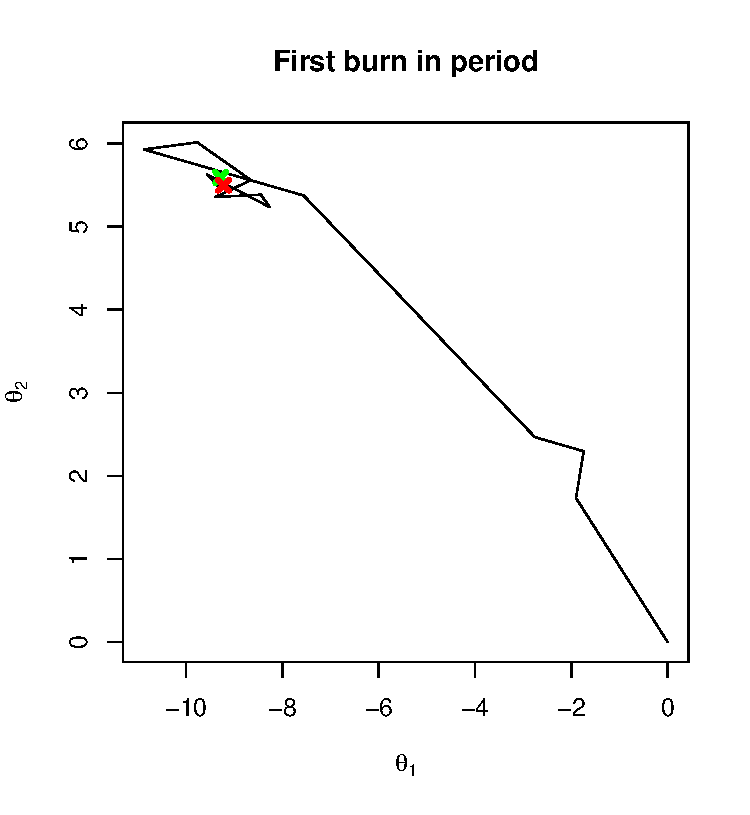
\includegraphics[width=0.49\textwidth]{figures/first-burn-in}
	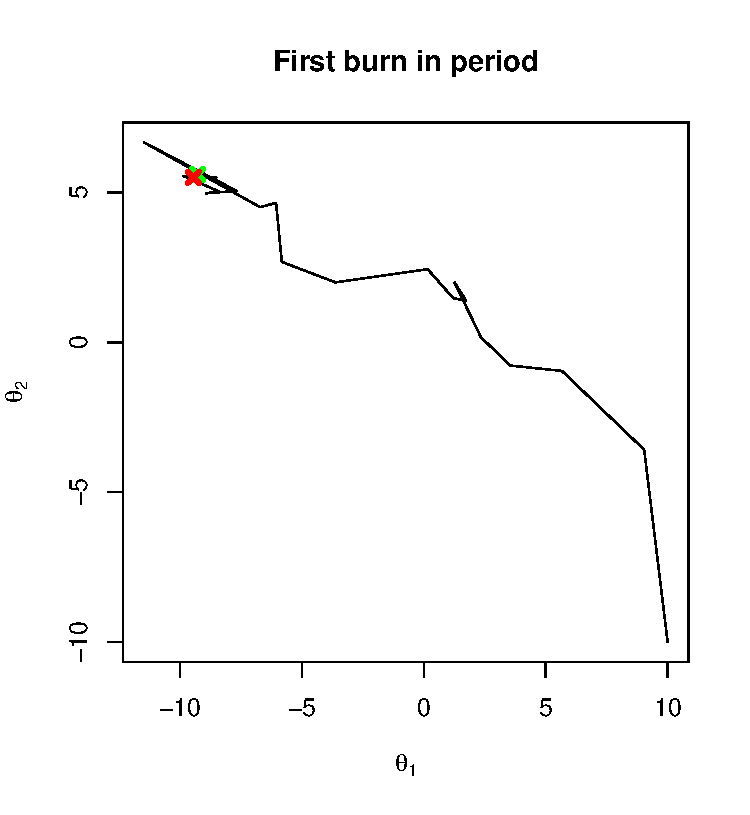
\includegraphics[width=0.49\textwidth]{figures/first-burn-in-second-start}
%	\tag{1}
	\caption{A plot of the first burn in period with two different starting points -- the origin and \((10, -10)\). The regularised MLE for the log linearity constant is marked by the green cross and the mean of the second half of the random walk by the red cross.}
	\label{fig:findingstart}
\end{figure}

Further the plots in Figure \ref{fig:MCplot} of the states of the Markov chain show that the acceptance rate drops significantly. This is a sign that we were successful in the process of finding an area with high density, since a lot of rejections imply, that the proposed points had all lower density. 

%In our case, the MH random walk focuses on the same region for all starting points and hence we will use this as a %Once we have run this first phase of burn in we see that the MH random walks all centered around a similar region independent from their starting point. Hence, we can choose one point in this region as the starting point of all further MCMC simulations.

\begin{figure}[h!]
	\centering
	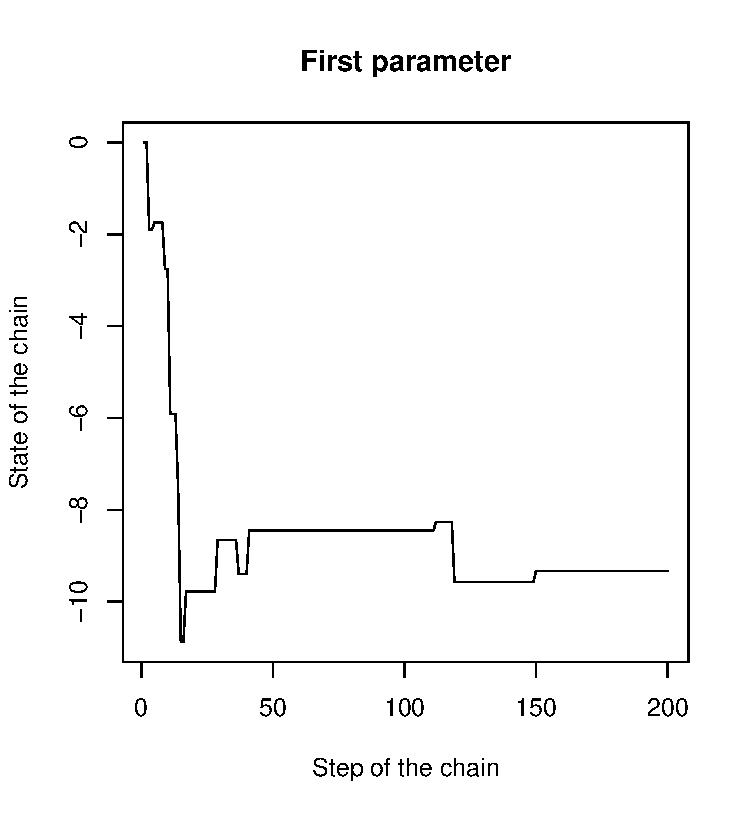
\includegraphics[width=0.49\textwidth]{figures/first-parameter}
	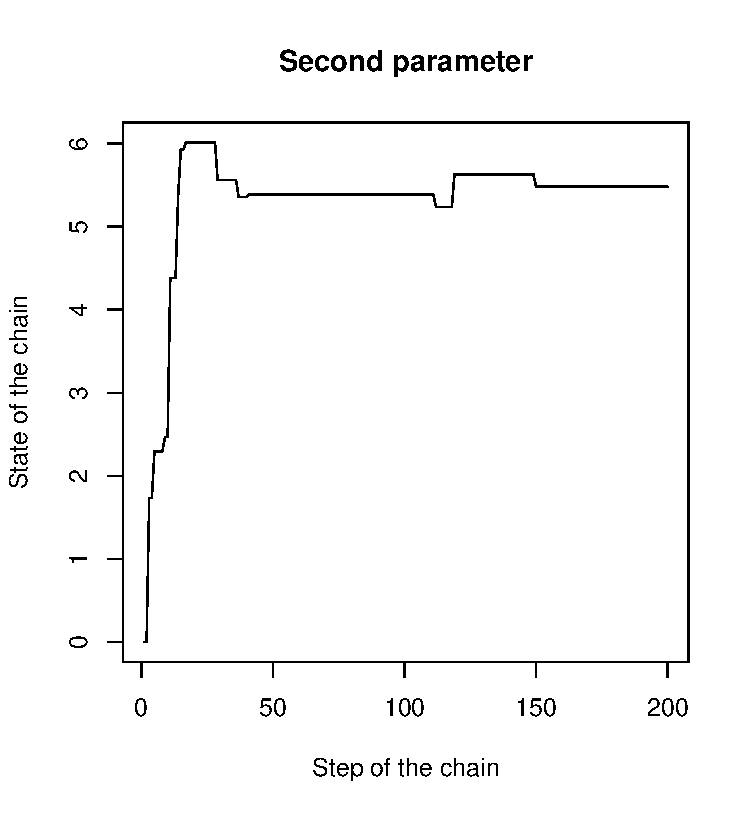
\includegraphics[width=0.49\textwidth]{figures/second-parameter}
%	\tag{1}
	\caption{Plots of the two state parameters of the MH random walk starting at the origin. The acceptance rate drops significantly and hardly any proposals are accepted.}
	\label{fig:MCplot}
\end{figure}

One could argue that it would be reasonable to choose the MLE as a starting point since for a very flat prior distribution it should also be approximately the mode of the posterior distribution. However, since we partly motivated the Bayesian approach to be an alternative to the infeasible maximum likelihood estimation for the elementary kernel \(L\), we presented the procedure above that can also be used for the estimation of \(L\).
\end{emp}

\begin{emp}[Second burn in to tune the proposal]
We use the second burn in method to tune the proposal according to \ref{tuning} for the final simulation. To do this we first select a starting point according to the result of the first burn in period. Then we adjust the variance of the Gaussian proposals such that we obtain a reasonable acceptance rate. This will be much lower than the one of the first burn in since we have seen in the state plots of the first burn in period that the acceptance rate decreased heavily. %The reason for this is, that if one uses a proposal with big variance and starts at a point with high density, then the proposal will mostly propose points far away from this point which will mostly have low denstities and therefore are likely to be declined. 
In a heuristic way it can be said that one now works �locally� and tries to explore the finer structure of the distribution and has to take smaller steps in order to do so.
We run this MH random walk for \(10^3\) samples and calculate their empirical covariance \(\Sigma\in\mathbb R^{2\times 2}\) and obtain the Markov chain depicted in \ref{fig:tuning}. We see that the points are located around the regularised MLE and we can get a first idea along which direction the parameter is more uncertain.


\begin{figure}%[h!]
	\centering
	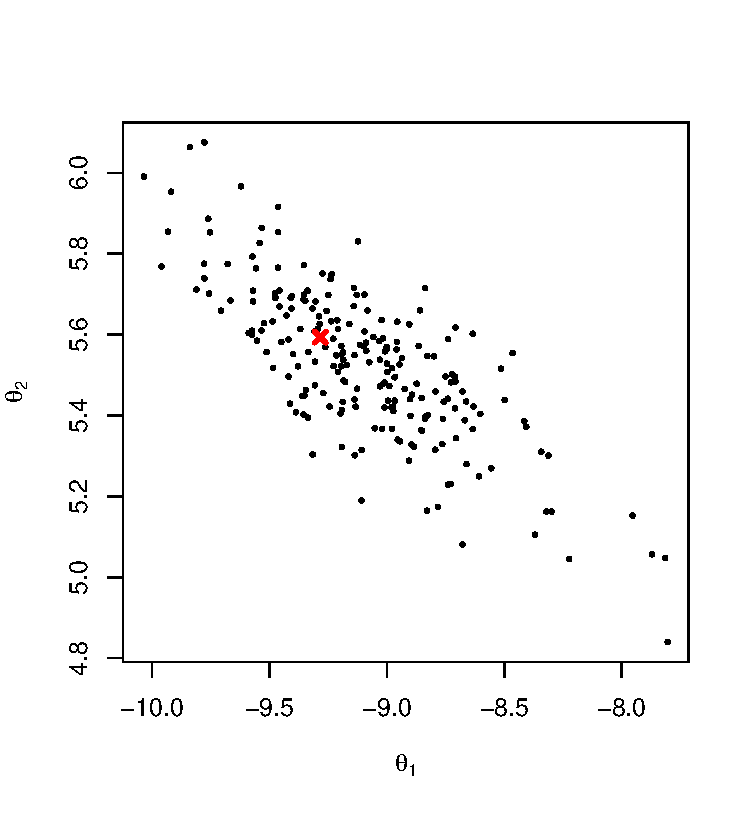
\includegraphics[width=0.55\textwidth]{figures/second-burn-in}
%	\tag{1}
	\caption{A plot of the samples of the MH of the second burn in period. One can see how the points are distributed around the MLE which is marked green. Their empirical covariance will be used to tune the proposal.}
	\label{fig:tuning}
\end{figure}
%\enlargethispage{1.5cm}
\begin{figure}[h!]
	\centering
	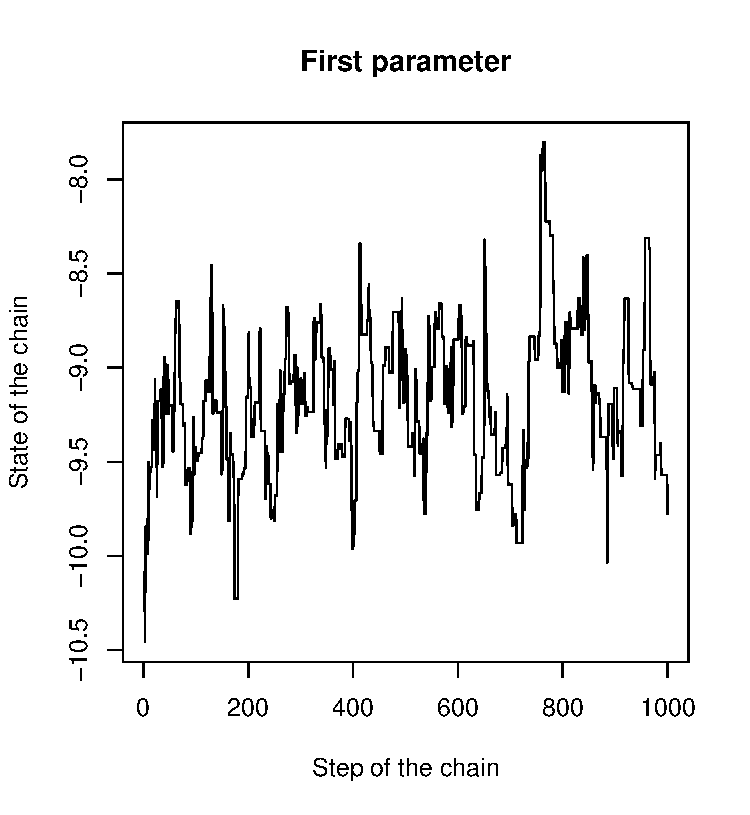
\includegraphics[width=0.49\textwidth]{figures/bayes-second-burn-in-first-parameter}
	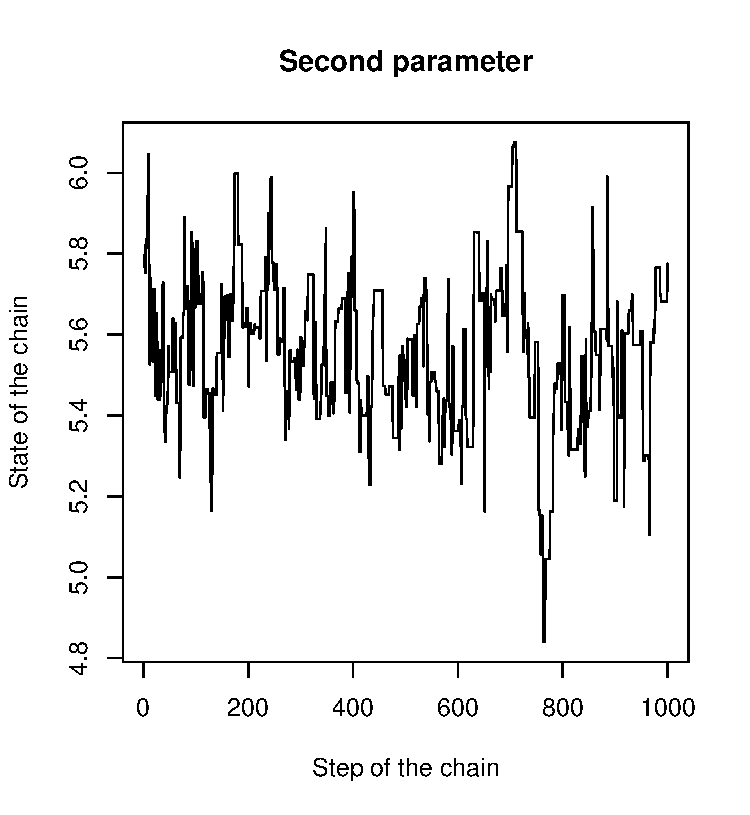
\includegraphics[width=0.49\textwidth]{figures/bayes-second-burn-in-second-parameter}
	%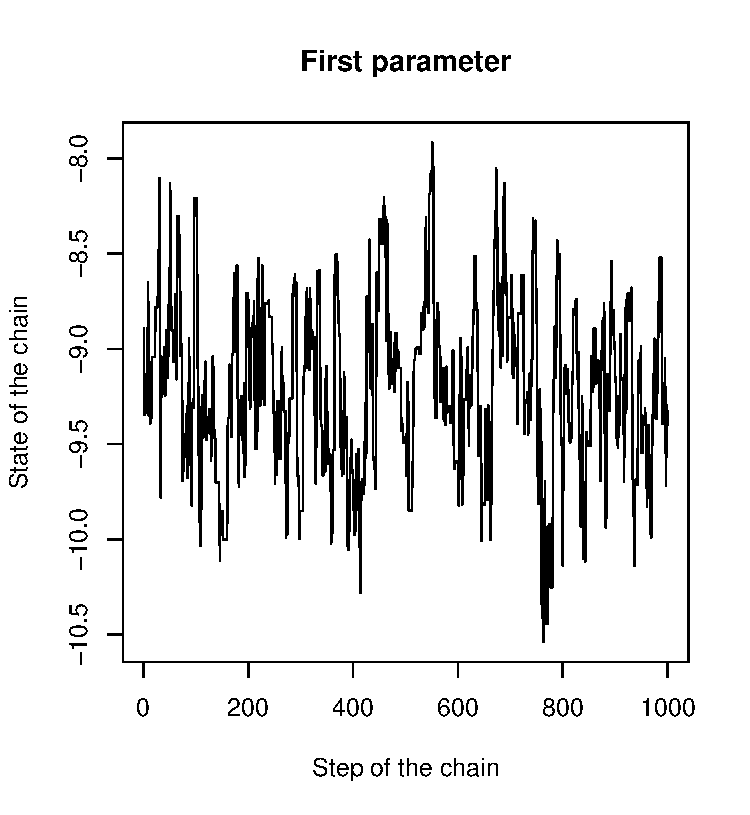
\includegraphics[width=0.49\textwidth]{figures/bayes-final-MH-first-parameter}
	%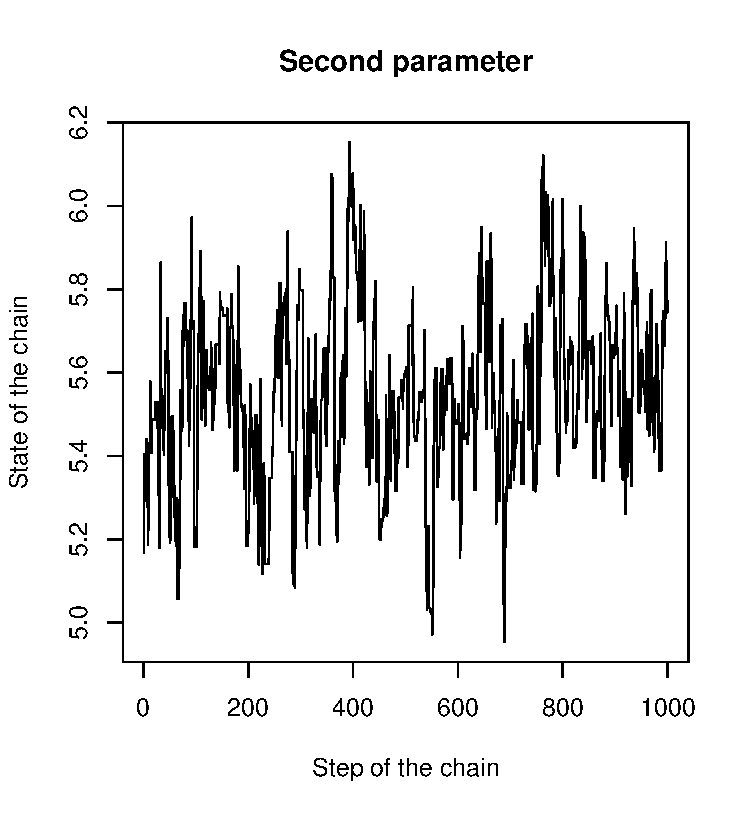
\includegraphics[width=0.49\textwidth]{figures/bayes-final-MH-second-parameter}
%	\tag{1}
	\caption{State plots of the second burn in period. One can see that the acceptance rate is a lot higher than in the first burn in.}
	\label{fig:mixim-tuning}
\end{figure}
\end{emp}

\begin{emp}[The actual MCMC simulation]
In this final step we run a MH random walk with length \(10^4\) and with the same starting point as in the second step. Now we use the prior adjusted according the second burn in period. This means we choose \(f(\cdot|\theta)\) to be the density of a normal distribution centered at \(\theta\) and with covariance \(\Sigma\). % This procedure adjusts the proposed steps into the diffrernt directions on the 
This leads to a higher acceptance rate of \(59\%\) compared to \(30\%\) in the second burn in period which can also be seen in the according state plots in Figure \ref{fig:mixim-tuning} and \ref{fig:mixim-tuning-final}. Further we see in Figure \ref{fig:acf-sbi-final} that the auto correlation function decreases faster with this tuned proposal.
\begin{figure}%[h!]
	\centering
	%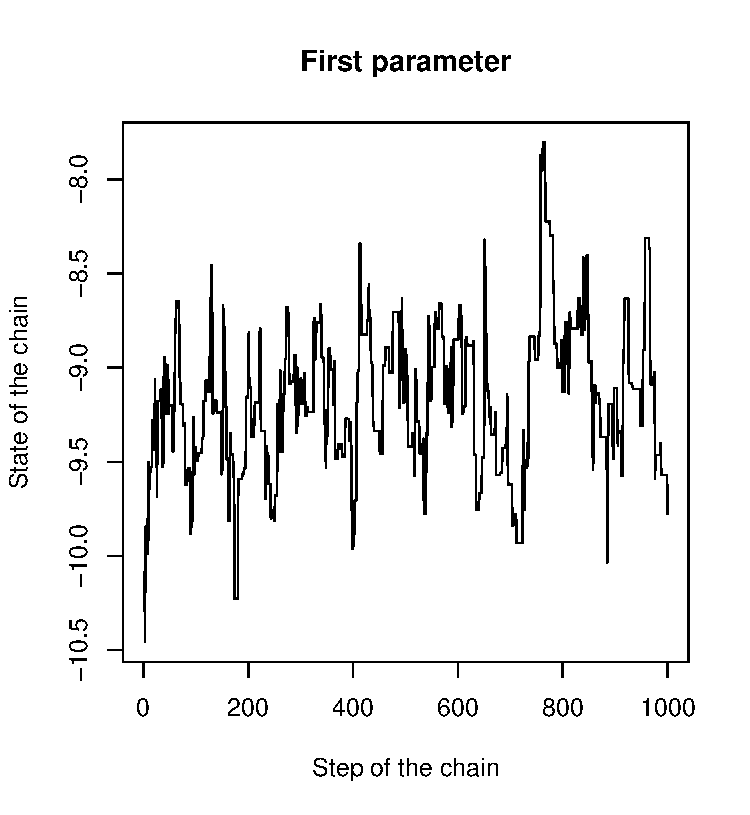
\includegraphics[width=0.49\textwidth]{figures/bayes-second-burn-in-first-parameter}
	%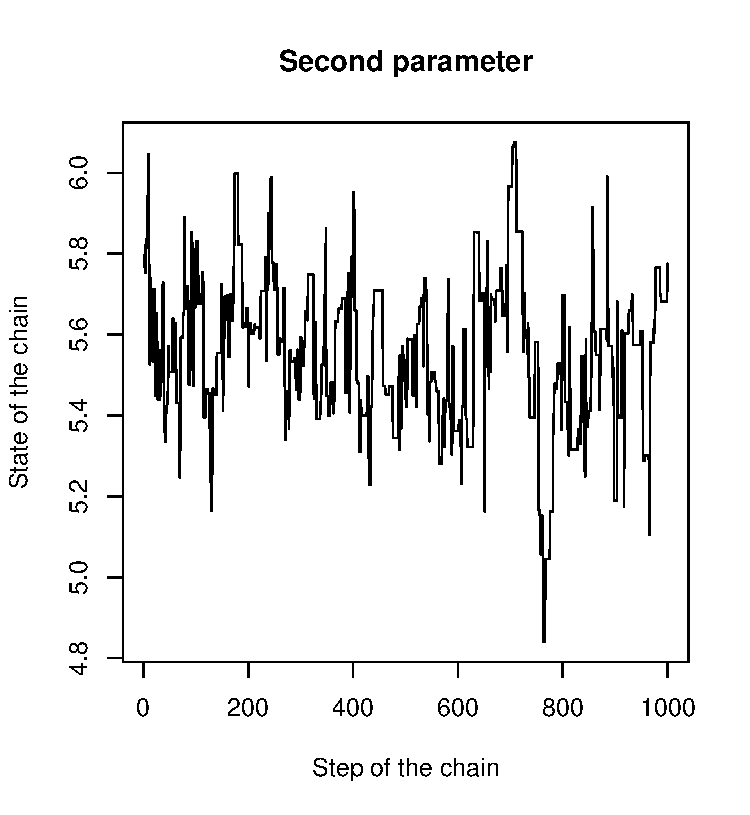
\includegraphics[width=0.49\textwidth]{figures/bayes-second-burn-in-second-parameter}
	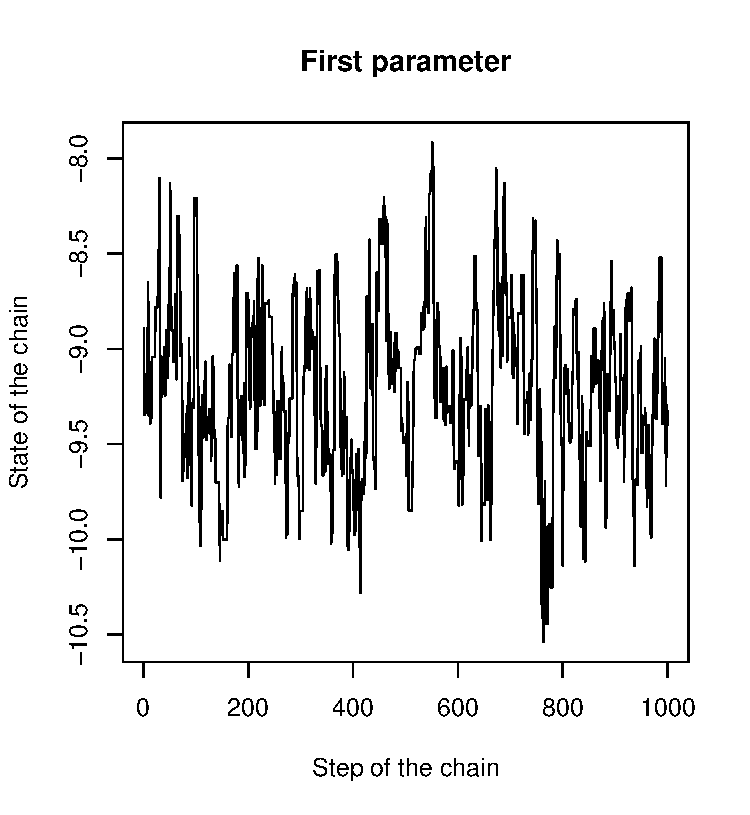
\includegraphics[width=0.49\textwidth]{figures/bayes-final-MH-first-parameter}
	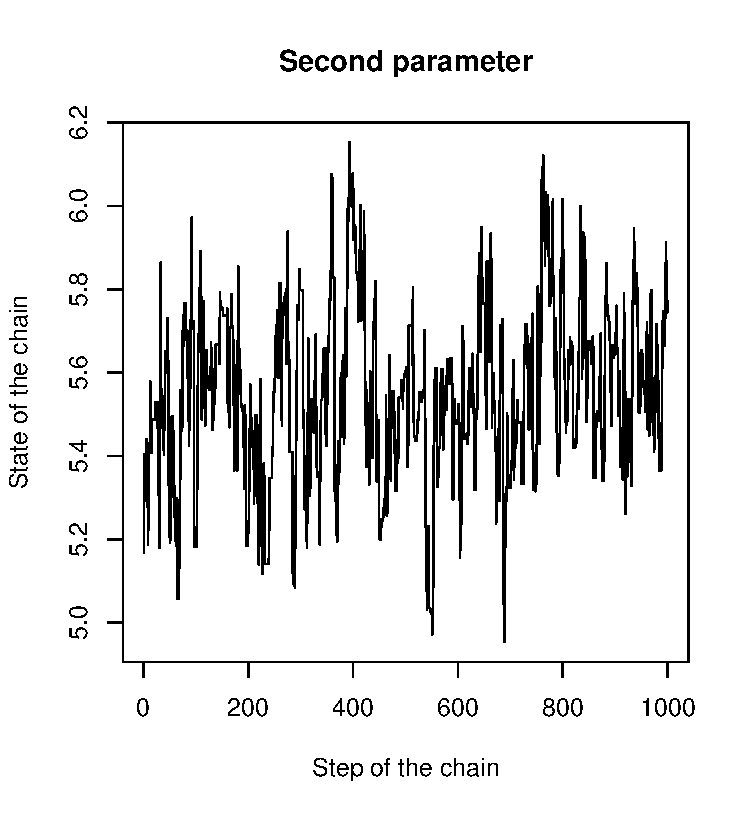
\includegraphics[width=0.49\textwidth]{figures/bayes-final-MH-second-parameter}
%	\tag{1}
	\caption{State plots of the %second burn in period on the top and the 
	final MH random walk on the bottom. One can see how the tuned proposal gives a higher acceptance rate than in the second burn in period.}
	\label{fig:mixim-tuning-final}
\end{figure}
\begin{figure}%[h!]
	\centering
	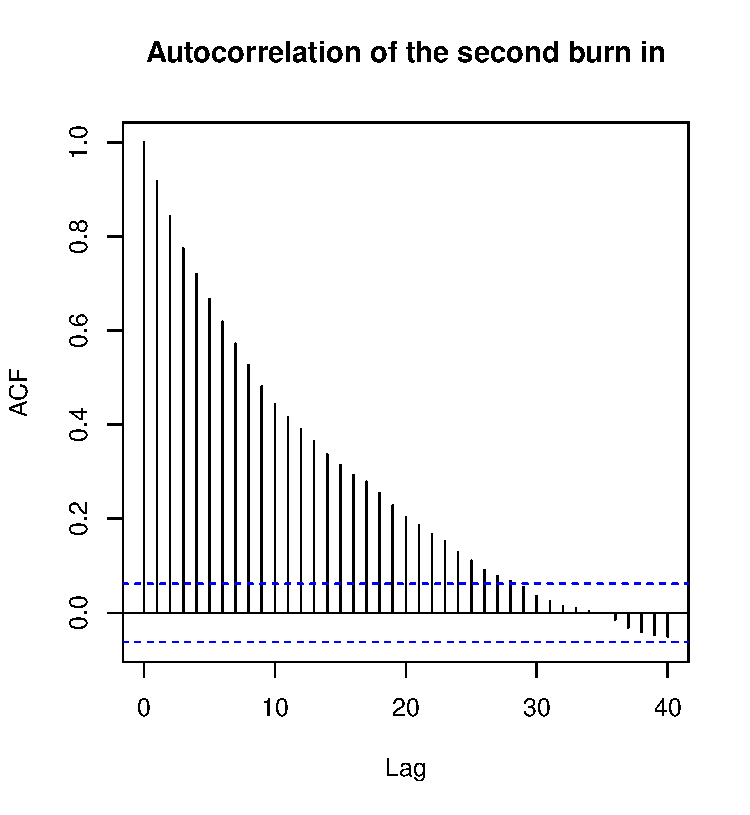
\includegraphics[width=0.49\textwidth]{figures/bayes-acf-second-burn-in}
	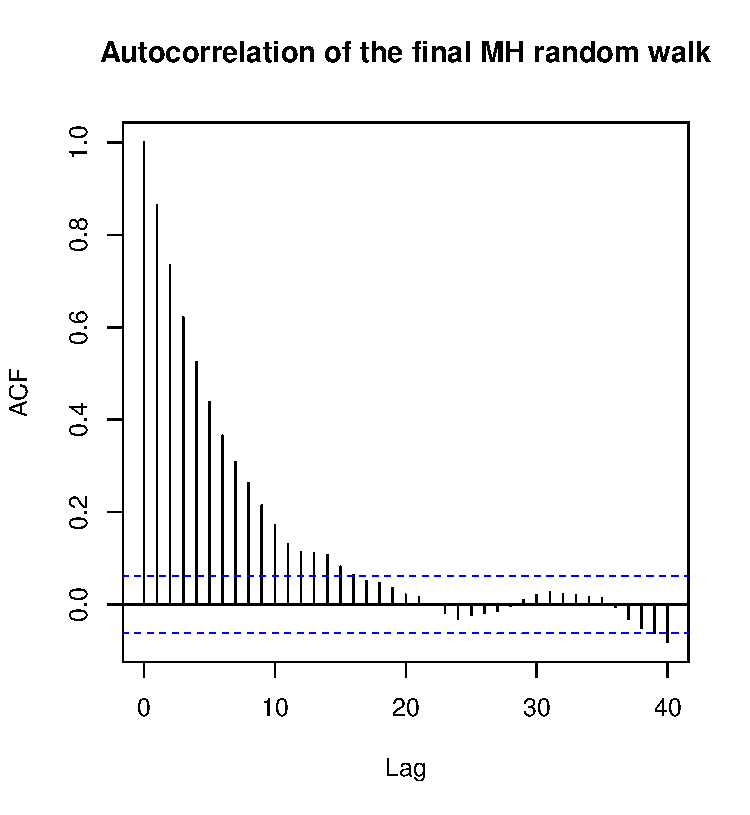
\includegraphics[width=0.49\textwidth]{figures/bayes-acf-final-MH}
%	\tag{1}
	\caption{A plot of the autocorrelation functions of the second burn in period and the final MH random walk. The latter one decreases faster which hints to a faster convergence due to the tuned proposal distributions.}
	\label{fig:acf-sbi-final}
\end{figure}
Finally we use a pre-implemented interpolation method to obtain a smoothed twodimensional histogram -- also called a heat plot -- which is shown in Figure \ref{fig:MHrw}.% \todo{does this make sense}% ....? %The resulting heat map can be seen in Figure \ref{fig:MHrw}.%recent\todo{say something about intuition}
\begin{figure}%[h!]
	\centering
	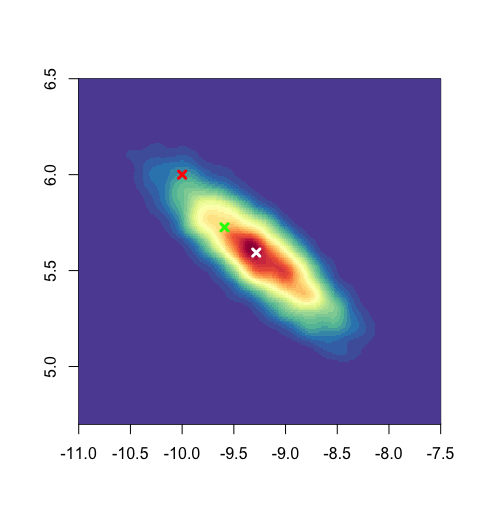
\includegraphics[width=0.55\textwidth]{figures/bayes-mle-and-regmle}
%	\tag{1}
	\caption{Heat map of the MH random walks with \(10^4\) iterations. The regularised MLE estimator is shown as a white, the MLE as a green and the actual parameter as a red cross. The regularised MLE is the maximum of the (approximated) posterior.}
	\label{fig:MHrw}
\end{figure}
\end{emp}

\subsubsection*{Bayesian approach without prior}

We have seen that the prior or regulariser influences the estimator and will often lead to worse estimates. However we have discussed shortly how we can follow a generalised Bayesian approach without a prior which results in having the likelihood function as a posterior,
\[f_{\Theta|X}(\theta|x) = f_{X|\Theta}(x|\theta).\]
In order to see that the MCMC approximation still works for this function, we note that
\[\mathrm{d}\pi \coloneqq f_{\Theta|X}\cdot\mathrm{d}\mu \]
is a \(\sigma\)-finite measure on the parameter space \(\Theta\). To approximate this measure, one can use the following more general version of the ergodic theorem.

\begin{theo}[Ergodic theorem]\label{ergTheo2}
Let \((X_n)_{n\in\mathbb N}\) be a Markov chain with \(\sigma\)-finite stationary distribution \(\pi\) and let 
\[\hat{\mathbb P}_n \coloneqq \frac1n \sum_{i=1}^n \delta_{X_i} \]
be the empirical measures associated with the Markov chain. Then the following two statements are equivalent:
\begin{enumerate}
\item For any \(\pi\)-integrable functions \(f, g\) with \(\int g(x)\pi(\mathrm{d} x)\ne0\) we have
\[\frac{\int f(x) \hat{\mathbb P}_n(\mathrm{d} x)}{\int g(x)\hat{\mathbb P}_n(\mathrm{d} x)} \xlongrightarrow{n\to\infty} \frac{\int f(x)\pi(\mathrm{d} x)}{\int g(x)\pi(\mathrm{d} x)}. \]
\item The Markov chain \((X_n)_{n\in\mathbb N}\) is  Harris recurrent.
\end{enumerate}
%, then \((X_n)_{n\in\mathbb N}\) is \emph{ergodic}. This means that if %\(\gamma_n\) be the distribution of \(X_n\), then we have
%\[\hat{\mathbb P}_n \coloneqq \frac1n \sum_{i=1}^n \delta_{X_i} \]
%is the empirical measure, we have almost surely have
%\begin{equation}\label{ergo}
%\int\limits_{\mathcal X} f(x) \hat{\mathbb P}_n(\mathrm dx) \xlongrightarrow{n\to\infty} \int\limits_{\mathcal X} f(x)\pi(\mathrm dx)
%\end{equation}
%for every \(\pi\) integrable function \(f\).
\end{theo}

%Obviously we can not normalise it in general since it does not need to be finite. However the ergodic theorem \ref{ergTheo} still holds for sigma finite measures and
This implies directly that the restrictions of \(\hat{\mathbb P}_n\) onto sets of finite measure \(\pi(A)<\infty\) converge weakly towards \(\pi\) up to normalisation. The argument for the stationarity of the \(\sigma\)-finite measure \(\pi\) stays exactly the same as before. 
\begin{figure}[h!]
	\centering
	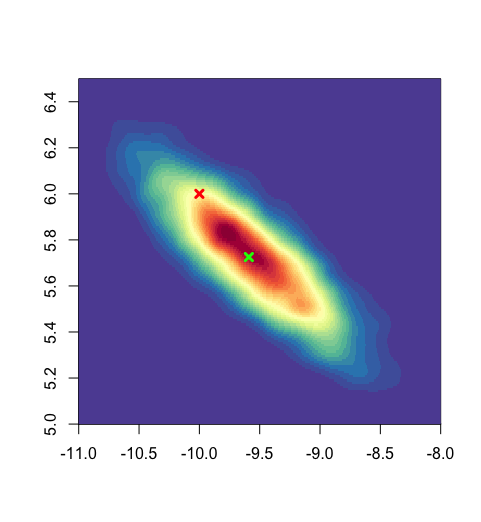
\includegraphics[width=0.6\textwidth]{figures/bayes-mle-withou-prior}
%	\tag{1}
	\caption{Heat map of the MH random walks with \(10^4\) iterations. The regularised MLE estimator is shown as a white, the MLE as a green and the actual parameter as a red cross. The regularised MLE is the maximum of the (approximated) posterior.}
	\label{fig:MHrwwup}
\end{figure}
Hence, we can take a completely analogue approach for the approximation of the likelihood function, but we only present the result of the third and final MCMC simulation in Figure \ref{fig:MHrwwup}.
%Further in the case of MLE it destroys the consistency of the estimation procedure. Where the MLE can easily be carried out without a regulariser, we have only seen how the Bayesian approach
%the Bayesian approach needs a prior. Unfortunately the uniform distribution, which corresponds to MLE without regularisation, does not exist on the parameter space \(\mathbb R^2\). If we use the uniform distribution on a sufficiently large -- meaning that it contains the MLE -- ball \(B_R(0)\subseteq\mathbb R^2\) as a prior, the mode of the posterior will be the MLE again.

%We choose such a uniform distribution and approximate the posterior just like before using a MH random walk. 

It is evident from both, theoretical considerations and the experimental results of the maximum likelihood estimations and the approximations of the posterior that the regulariser or prior always forces the estimation to get closer to the origin. Obviously this can make the estimation better, if for example the unregularised MLE is larger than the actual parameter, but then it makes the estimation better by pure luck. We will see later that the influence of the prior is a little bit more positive if the data is perturbed by random noise.

\subsubsection*{A naive approximation of the posterior}

The motivation for the use of MCMC methods was that one wants to obtain an approximation of the posterior. We present here a different and naive approach, which works a lot faster and with higher accuracy. However we will see later that this approach suffers from what is known as the \emph{curse of dimensionality},\footnote{This name is used for pretty much all phenomena that grow exponentially with the dimension of the problem.} i.e. the time needed to perform it will grow exponentially with the dimension of the parameter that should be estimated.

Let us assume that we have performed the two burn in periods of the MH random walk presented above. Then we roughly know the location of the high density from the first burn in period and also the approximate shape of it from the second one. Now we place a \(40\times 40\) grid above this box and evaluate the unnormalised posterior at those grid points. Then we use an interpolation algorithm to obtain an approximation of the unnormalised posterior density. This interpolation usually comes in a quite simply form -- for example piecewise linear -- and can therefore by explicitely expressed and integrated in order to normalise the approximate posterior. The results for this approach can be seen in Figure \ref{fig:directHeatMaps} and we will discuss the advantages and hindrances in the next paragraph.

\begin{figure}[h!]
	\centering
	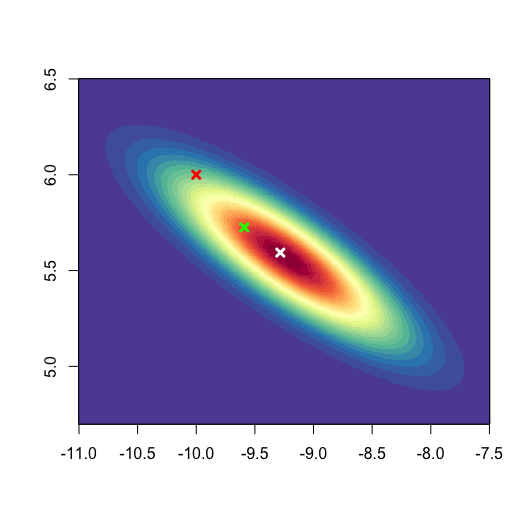
\includegraphics[width=0.49\textwidth]{figures/posterior-direct-approx}
	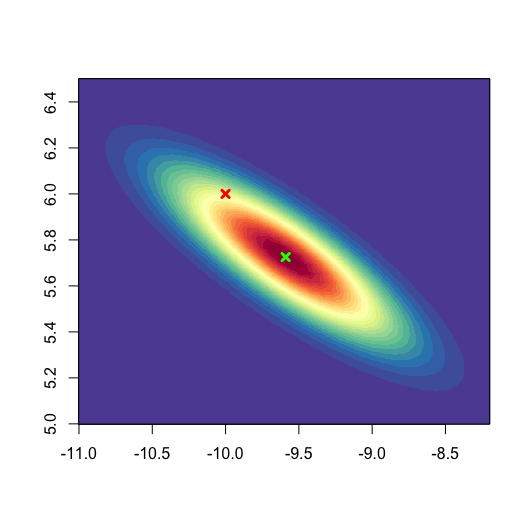
\includegraphics[width=0.49\textwidth]{figures/likelihood-direct-approx}
%	\tag{1}
	\caption{Approximations of the posterior (on the left) and of the likelihood function (on the right) obtained by the interpolation between breakpoints. Just like in the approximations using MCMC methods, the reguralised MLE is marked white, the MLE green and the actual parameter red.}
	\label{fig:directHeatMaps}
\end{figure}

\subsubsection*{Complexity of the different approaches}

In large examples the evaluation of the likelihood function
\[f_{X|\Theta}(x|\theta) \propto \prod_{i=1}^n \frac{\det(L(\theta)_{A_i})}{\det(L(\theta) + I)} \]
involves the computation of a \(N\times N\) matrix. This can be done explicitly using Gauss elimination which does not change the determinant -- at least up to a sign -- and can be performed in at most \(N^3\) steps, cf. \cite{valiant1979complexity}.\footnote{Actually one can even do better, but those algorithms come with greater implementation challenges.} Hence, the time neede for the computation of the likelihood function can be bounded -- up to a constant -- by
\[N^3 + \sum_{i=1}^n \left\lvert A_i \right\rvert^3 \le (n+1) \cdot N^3\]
and we say it can be performed in \(O(N^3)\) 
%\[O\left( N^3 + \sum_{i=1}^n \left\lvert A_i \right\rvert^3\right)\]
time.\footnote{See also the Landau or �big \(O\)� notation in the nomenclature.} 
In practice this will take a significant amount of time and this was also the motivation for the variational MCMC methods. For example in our toy example the computation took between one and two seconds on a six year old \(1.8\si{GHz}\) Intel Core i5 using the determinant algorithm in R.

For a single step of the MH random walk the unnormalised posterior needs to be evaluated twice for the computation of the acceptance threshold \(\rho(x, y)\), cf. \eqref{threshold}. Usually one will work with a prior that is easy to compute and with a proposal that can be simulated fast and hence we will neglect its contribution and hence one step of the performance of one MH random walk can be carried out in \(O(N^3)\) time. If \(T\) denotes the length of the MCMC method, the time needed for its simulation is 
\begin{equation}\label{complexityMCMC}
O\left( T\cdot N^3\right).
\end{equation}

In the final step of the MH random walk, we set \(T=10^5\) as the length and this relates to an approximate simulation time of
\[10^5 \cdot 2\cdot 1.5\si{s} = 3\cdot10^5 \si{s} \approx 8\si{h}.\]
The strength of the naive approximation based on the interpolation between breakpoints is that one only has to evaluate the unnormalised posterior \(40^2 = 1.6\cdot10^3\ll 10^5\) times. The time needed for this is approximately
\[1.6\cdot10^3 \cdot 1.5\si{s} = 2.4\cdot 10^3 \si{s} = 40\si{min}. \]
However, % the results shown in the Figures \ref{fig:MHrw}, \ref{fig:MHrwwup} and \ref{fig:directHeatMaps} suggest that the approximation gained by this direct approach are more accurate\todo{find an argument for this}, not everything is perfect. In fact, 
if we denote the dimension of the parameter by \(M\), then the size of the grid of breakpoints needed for the interpolation grows exponentially in \(M\). Let \(R\) denote the number of grid lines along each coordinate, then one needs to evaluate the posterior \(R^M\) times and the times for this behaves like
\begin{equation}\label{complexityDirect}
O\left( R^M\cdot N^3\right).
\end{equation}
In \(10\) dimension and with \(40\) grid lines along all dimensions, this corresponds to \(40^{10} > 10^{16}\) evaluations which can not be performed in reasonable time. This exponential increase makes this direct approach only impossible if the parameter one wishes to estimate is not very low dimensional. Nevertheless it might be possible to modify this approach in a suitable way to make it more promising in higher dimension. For example one could try to iteratively raise the resolution of the grid on the places where one expects a high value of the function or high changes of the function. Alternatively it might be worth to investigate how different approximation algorithms of high dimensional functions could help in this approach.

It shall be noted that also the method of numerical integration suffers from the course of dimensionality since numerical integration relies on the evaluation of the function on an exponentially increasing number of points.
\todo{How does \(T\) grow with \(M\)?}

The complexity of the slice sampling algorithm can not be given this easily, at least for the version we presented. This is because the approximate sampling from the uniform distribution on the slice proposed in Algorithm \ref{alg:slice-sampling-implementation} can need arbitrarily many samples from the uniform distribution on the proposed cuboid. Although those uniform samples can be generated efficiently one has to evaluate the unnormalised posterior each time to check whether the proposed sample is actually contained in the slice.
%\todo{comment on complexity for silce sampling?}
 %The comparison to \eqref{complexityMCMC} shows that the direct approach is only 
 


\subsubsection*{Comments on real world applications}

Although this is just a controlled toy example, this procedure can easily be generalised to real world settings. However, one has to face the following two major challenges:
\begin{enumerate}
\item In practice one will not know the feature vectors \(f_i\) like we did, so one will have to model those. Usually one would put all quantitative properties into this vector that one would believe could have an effect on the quality of an item. For example if the DPP should model the picnic positions of people in a park one could argue that the quality, i.e. the popularity of a picnic spot depends amongst other things on the distance to the next trash bin, the next toilet and overall noise level. Although one thinks that those parameters can play a role, we could not argue a priori whether they have a positive or a negative impact. For example if the toilets are nice and clean it might be favourable to be closer to them, if they are dirty it might be better to be far away from them in order to avoid their unpleasant odour. However, one does not have to know this straight away as this effect is determined by the according log linearity constant and hence can be estimated in the above manner.
\item Secondly and maybe even more importantly the actual similarity kernel is also unknown and hence one also has to come up with a reasonable model for it. Either this can be done by purely relying on models created by people familiar with the real world phenomenon that is being investigated, or one could also try to estimated the similarity kernel itself. However, estimating the whole similarity kernel is equivalent to a maximum likelihood estimation of the whole elementary kernel \(L\) and we have seen in the previous discussion about computability that this results in an optimisation problem that can not be solved efficiently. However, we will propose a different, possibly more practical approach in the next section, but it still remains to be seen whether this will actually give any benefits.
% a more subtle approach would be to assume that the diversity feature vectors \(\phi_i\) have the form 
%\[(\phi_i)_j\propto f( \sigma \left\lVert i - j \right\rVert) \quad \text{for } i, j\in\mathcal Y\]
%and then try to estimate the parameter \(\sigma\). With this approach one would only have to estimate one additional parameter instead of the \(N^2 = 900\) parameters of the similarity kernel \(S\). However, with this approach the log likelihood function is likely to be non concave and hence it remains to investigate whether there are any other efficient optimisation techniques for it. \todo{think more towards this direction}
\end{enumerate}


\section{Stability under noise -- does the regularisation help?}

In real world applications the observed data will almost never be free from noise and outer influences. Therefore one wants to establish stable estimation techniques in the sense that small changes in the data should only lead to small changes in the estimation. This is nothing but the question of continuity of the estimation rule and in a lot of scenarios a regulariser or prior can help to lower the effect that random perturbations of the data have on the estimation, cf. \cite{buhlmann2011statistics}. %This is typically necessary if the estimation is very instable, i.e. if small changes in the observation lead to big changes in the estimated parameter. 
Thus, we want to investigate whether this is the case for  the parameter estimation of discrete DPPs. First we have to specify what noise we are going to consider in the case of discrete DPPs. If one works with continuous DPPs one could assume a perturbation of the exact positions of the observed points, however in the discrete setting this does only make limited sense. Therefore we will work with the observations of a DPP where points are randomly added or deleted and will specify this later.

Before we investigate the stability properties of the estimation in the specific setup for DPPs, we should make a general statement. The estimation can be seen as the following two stage process
\[\text{data } x\; \xlongrightarrow{\text{evaluation of } f_{X|\Theta}}\; \text{posterior } f_{X|\Theta}(x|\cdot) f_\Theta(\cdot)\; \xlongrightarrow{\text{maximisation}}\; \text{MAP estimator } \hat \theta. \]
%\[\text{data}\; \xlongrightarrow{\text{evaluation of } f_{X|\Theta}}\; \text{posterior}\; \xlongrightarrow{\text{maximisation}}\; \text{MLE}. \]
If one wants to investigate the stability properties of the estimation which is nothing but the continuity, then it is reasonable to do this for both steps separately. The second step is in general discontinuous since the maximisation of a function is not a continuous operation under the usual topologies on functions corresponding to uniform or pointwise convergence or integral norms. 
%Because of this factorisation, it is immediate that the if the % posterior density has a better stability property that the MLE, since 

Usually the first step will be continuous in some notion, for example if all densities \(f_{X|\Theta}(x|\theta)\) are continuous in \(x\), then the posterior depends continuously on the data \(x\) in terms of pointswise convergence which corresponds to the product topology. The choice of the prior can possibly strengthen this continuity property and lead to a uniform convergence. If additionally all posterior densities have a unique maximiser, then the maximisation is continuous on this subclass of functions with respect to the uniform topology. In summary we have seen that the prior comes into play at two points, the first one to strengthen the continuity of the first step and then to lead to a possibly more well behaved class of posterior densities. %The continuity properties of the first step are influenced by the prior and 

%\begin{emp}[The trouble with discrete data]
In the case of discrete DPPs, our space of observations \(2^\mathcal Y\) is discrete and hence the only reasonable topology on it is the discrete topology, i.e. the powerset itself. Every mapping is continuous with respect to this topology and hence the prior is not needed for this qualitative property. Thus, there is no apparent reason why the regularisation or the prior should bring any benefit. % it -- with no presence of noise -- pushes the estimator towards the center of the prior distribution which is the origin in our toy example.
We will see in our examples that it can actually be used to regularise certain parameters of the DPP but only if one has a very clear understanding of how those parameters are influenced by the noise. %We will additionally run experiments with noisy data to confirm our claim that the regularisation or prior introduces a bias\todo{explain this term}{ } for one parameter and can be used for the regularisation of the second parameter since the noise affects the cardinality of the DPP. % of the estimation without making the estimation more stable unless in the presence of extreme noise.
%\end{emp}



%\begin{emp}[General comment on ]

%\end{emp}

%\begin{emp}[Regularisation of the quality]

%\end{emp}

%\begin{emp}[Regularisation of the kernel]

%\end{emp}

\subsubsection{Experiments}

First we explain which kind of noise we will consider.

\begin{emp}[Setting]
Let \(B_1, \dots, B_n\) be independent realisations of a DPP \(\mathbb P\). Let further \(C_1, \dots, C_n\) be independent  realisations of an independent Poisson point process. We assume that we have given the data
\[A_i \coloneqq B_i\setminus C_i\cap C_i\setminus B_i \quad \text{for } i = 1, \dots, n. \]
The observations \(A_i\) correspond exactly to the observation of a DPP where points were randomly deleted and added.
\end{emp}

We will generate noisy data consisting of \(n=8\) samples of a DPP perturbed by a Poisson point processes with marginal kernel \(\rho\cdot I\) where we call \(\rho\in(0, 1)\) the \emph{intensity} of the point process.
%with different cardinalities and
We calculate the MLE and regularised MLE corresponding to the regularisation given by the prior \eqref{toyprior}. 
%More precisely we will work with Poisson point processes with different marginal kernel \(\rho\cdot I\) where we call \(\rho\in(0, 1)\) the \emph{intensity} of the point process. The intensity corresponds to how likely points are dropped from and added to the DPP.
We use an intensity of \(\rho=\frac1{400}\) and run repeat this procedure eight times and the results of this are fixed in Table \ref{tab:MLEvsRegMLE}.

\begin{table}[h!]
\centering
\begin{tabular}{ |c|c|c|c| } 
 \hline
  & MLE %with intensity \(\rho=\frac1{400}\) 
  & regularised MLE & %with intensity \(\rho=\frac1{400}\) 
  \\ \hline
 1 & (-10.05, 7.22) &  (-9.76, 7.09) & \\ \hline
 2 & (-9.44, 6.67) & (-9.16, 6.55) & \\ \hline
 3 & (-10.51, 7.05) & (-10.20, 6.91) & \\ \hline
 4 & (-9.79, 6.45) & (-9.49, 6.32) & \\ \hline
 5 & (-11.03, 7.06) & (-10.70, 6.92) & \\ \hline
 6 & (-10.07, 6.97) & (-9.78, 6.85) & \\ \hline
 7 & (-10.04, 6.53) & (-9.74, 6.40) & \\ \hline
 8 & (-9.76, 6.83) & (-9.47, 6.70) & \\ \hline
\end{tabular}
\caption{Table with the MLE and regularised MLE for noisy data perturbed by a Poisson point process with intensity \(\rho = \frac1{400}\).} \label{tab:MLEvsRegMLE}
\end{table}

Like in the case of estimation without noise, the regularised MLE is closer to the origin than the unregularised one. In the first component, this leads to worse estimates and in the second one to better ones. The reason that the estimation of the second parameter benefits from the regularisation is the following. If the cardinality of the DPP is smaller than \(N/2\), then the presence of noise -- at least the one we are considering -- leads to a higher expected cardinality in the data since more points are added than deleted because we expect
\[\left\lvert A_i\cap B_i  \right\rvert \le \left\lvert B_i \setminus A_i \right\rvert.\]
This leads to an estimation of higher qualities and the magnitude of the qualities is controlled through the second parameter. Hence, the regulariser forces the second component MLE into the right direction\todo{make this more scientific}. However this kind of regularisation can only be successful, if one has a clear understanding into which direction the noise will perturb the estimates. If for example the cardinality of the DPP is larger than \(N/2\) the Poisson noise will lower the cardinality of the data and the regulariser could increase this effect instead of weakening it. To decide whether the DPP has cardinality smaller or bigger than \(N/2\) one can use the observed data because if the intensity of the noise is lower than \(0.5\), then the expected cardinality of the observations remain smaller or larger than \(N/2\). To see this, assume the sample from the actual DPP satisfies \todo{?}%\(\)
%This is because of
%\[\]

Now that we have understood how the noise influences the two parameters, we can actually propose a different prior that is adapted to this. 
%Namely, it should be more appropriate to use a prior that only relies on the second parameter and regularises the estimation for this to become smaller. 
Hence, we use the adjusted prior
\[\tilde f_\Theta(\theta) \coloneqq \exp\left(-\frac{\theta_2^2}{2^4}\right) \]
which should only regularise the second the parameter. The improved results of this regularisation can be found in the Table \ref{tab:MLEvsRegMLE} on the very right. \todo{do this}

%However, this is only due to the fact that the cardinality of the DPP is much smaller than \(N/2\) in our case and if it was bigger, the estimation would be forced into the opposite way. In summary the prior can be used to regularise the second parameter which controls the cardinality of the DPP, but this must be done with a certain amount of care and under consideration whether the observed data is definitely smaller or bigger than \(N/2\).



%\begin{center}
%\begin{table}
%\centering
%\begin{tabular}{ |c|c|c| } 
% \hline
%  & MLE %with intensity \(\rho=\frac1{400}\) 
%  & regularised MLE %with intensity \(\rho=\frac1{400}\) 
%  \\ \hline
% 1 & () &  () \\ \hline
% 2 & () & () \\ \hline
% 3 & () & () \\ \hline
% 4 & () & () \\ \hline
% 5 & () & () \\ \hline
% 6 & () & () \\ \hline
% 7 & () & () \\ \hline
% 8 & () & () \\ \hline
%\end{tabular}
%\caption{This is my one big table} \label{tab:sometab}
%\end{table}
%\end{center}


%For example we could suppose that we want to estimate the coefficients of a polynomial based on some evaluations that are pertubed by random noise. Let�s say \(p_0 = 2x + 3\) is the polynomial we want to estimate based on \(n=9\) observations of the form \(p_0(x_i) + \varepsilon_i\) where \(x_i\) are real numbers and \(\varepsilon_i\) is a pertubation. We work with the following dataset:
%\begin{center}
%\begin{tabular}{ |c|c|c|c|c|c|c|c|c|c| } 
% \hline
% \(x\) & 1 & 2 & 3 & 4 & 5 & 6 & 7 & 8 & 9 \\ \hline
% \(y\) & 5 & 7 & 9 & 11 & 13.3 & 15 & 17 & 19 & 21 \\
% \hline
%\end{tabular}
%\end{center}

%Obviously the data is described the best way through the interpolating Lagrange polynomial -- this corresponds for example to the extremal estimator that minimises the distance of the function evaluated at the \(x\) values to the data. However it can be seen in Figure \ref{fig:instability} that this is a rather bad description of the actual underlying principle behind the data. 

%\begin{figure}[h!]
%	\centering
%	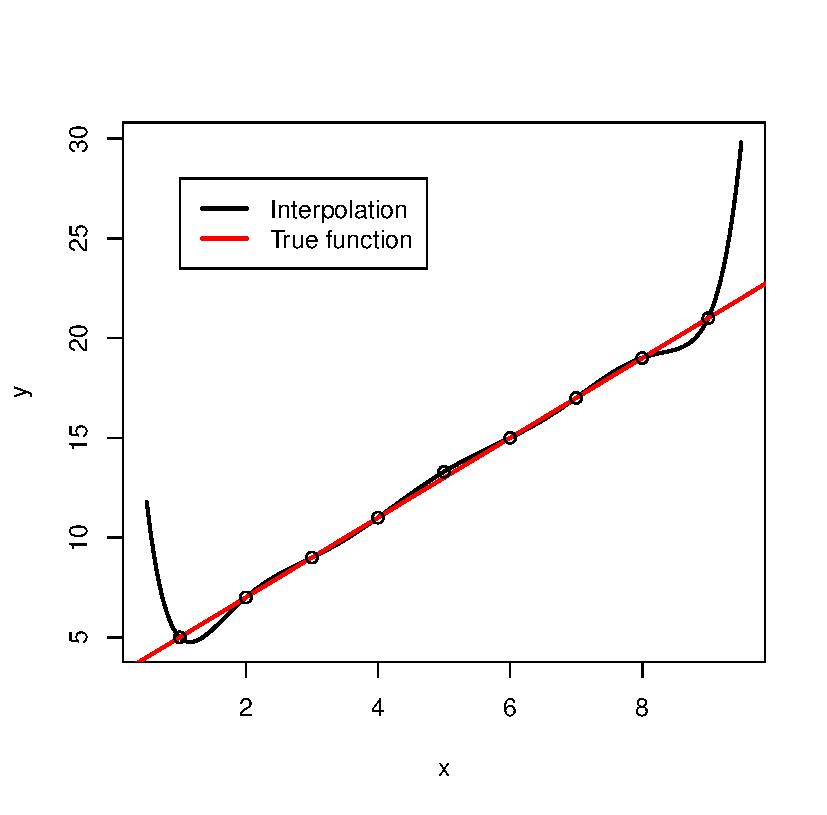
\includegraphics[width=0.6\textwidth]{figures/instability}
%	\tag{1}
%	\caption{Approximations of the posterior (on the left) and of the likelihood function (on the right) obtained by the interpolation between breakpoints. Just like in the approximations using MCMC methods, the reguralised MLE is marked white, the MLE green and the actual parameter red.}
%	\label{fig:instability}
%\end{figure}

%The problem is -- heuristically speaking -- that the interpolation is so irregular that it not only describesCalculus of Variations the underlying function, but also the noise. In this case a regulariser can be used to penalise irregular models, in this case the polynomials with high degree.




%\section{Towards deep DPPs}

%\section{A Bayesian approach to the kernel estimation}